\documentclass{jarticle}
\usepackage[dvipdfmx]{graphicx}
\usepackage{url}
%追加
\usepackage{listings}
\usepackage[dvipdfmx]{xcolor}
%\jintercharskip=0pt plus1.2pt minus0pt

\renewcommand{\baselinestretch}{1}
\setlength{\textheight}{25.5cm}
\setlength{\textwidth}{16.0cm}
%\setlength{\marginparsep}{0mm}
%\setlength{\marginparwidth}{0mm}
\setlength{\oddsidemargin}{0mm}
\setlength{\evensidemargin}{0mm}
\setlength{\headheight}{0mm}
\setlength{\headsep}{0mm}
%\setlength{\footheight}{10mm}
\setlength{\footskip}{10mm}
\topmargin=-5mm
\footskip=1cm
\setcounter{topnumber}{10}
\setcounter{bottomnumber}{10}
\setcounter{totalnumber}{10}
\renewcommand{\topfraction}{1.0}
\renewcommand{\bottomfraction}{1.0}
\renewcommand{\textfraction}{0.0}
\renewcommand{\floatpagefraction}{0.8}
\renewcommand{\floatsep}{8mm}
%プログラム挿入の設定
\usepackage{listings,jvlisting}
\lstset{
  basicstyle={\ttfamily},
  identifierstyle={\small},
  commentstyle={\smallitshape},
  keywordstyle={\small\bfseries},
  ndkeywordstyle={\small},
  stringstyle={\small\ttfamily},
  frame={tb},
  breaklines=true,
  columns=[l]{fullflexible},
  numbers=left,
  xrightmargin=0zw,
  xleftmargin=3zw,
  numberstyle={\scriptsize},
  stepnumber=1,
  numbersep=1zw,
  lineskip=-0.5ex
}

\usepackage[dvipdfmx]{graphicx}
\usepackage{colortbl}
\usepackage{here}
\usepackage{empheq}
\usepackage{cases}

\title{組み込みシステムレポート}
\author{明星大学情報学部情報学科\\
  20J5-141:渡部 皓太郎} %% 学籍番号・氏名
\date{提出日:2022年1月26日} %% 提出日


\begin{document}

\maketitle



\section{実験装置}
\begin{itemize}
    
    \item 装置名称
     \begin{itemize}
         \item 備わっている機能
     \end{itemize}
    
    \item レーザ光XY駆動ユニット
    \begin{itemize}
        \item X軸駆動サーボモータ
        \item X軸用ミラー
        \item Y軸駆動サーボモータ
        \item Y軸駆動ミラー
        \item Y軸用ミラー
        \item レーザポインタ
        
    \end{itemize}
    \item マイコンボード
    \begin{itemize}
        \item マニピュレータ接続端子
        \item XY駆動ユニット接続端子
        \item 汎用LED
        \item 電源表示LED
        \item 電源スイッチ
        \item インターフェースボード
        \item LAN端子
        \item マイコンボード
    \end{itemize}

    \item マニピュレータ
    \begin{itemize}
        \item アナログ値入力つまみ(X,Y軸)
        \item 押しボタンスイッチ(1,2)
    \end{itemize}
\end{itemize}


\section{課題1}
\subsection{目的}
マニピュレータのポテンシャルメータXとプッシュスイッチsw1の値を読み取り、コンソールに表示させる。


\subsection{実験方法}

potXandsw1を作成し実行した。

\begin{lstlisting}[caption=PotXandsw1]

import hardware.*;  //実験で実機を使用する場合にはコメントを外してこれを使用する
//import stub.*;  //予習などで実機を使用せずに動作を確認する場合には、これを使用する

public class Kadai1_PotXandSw1
{
    Hardware hardware = Hardware.getInstance(); //ハードウェアのインスタンスを取得する
    public void dispPotXandSw1() {

        while ( true ) {  //無限に繰り返す
            int potXvalue = hardware.manipulator.potX.getValue();
            //ポテンショメーターXの値を取得する
            System.out.print( "PotX = " + potXvalue );    //potXの値を表示する
            System.out.print( "     " );                    //表示での適度なスペースをとる
            System.out.print( "SW1 = " );
            if ( hardware.manipulator.sw1.isPush() ) {    //sw1が押されているか調べる
                System.out.print( "Pushed" );       //押されていたら「Pushed」と表示する
            } else {
                System.out.print( "Released" );  //押されてなければ「Released」と表示する
            }
            System.out.println();       //改行する
        }
    }
}

\end{lstlisting}

\subsection{結果}
表\ref{kadai1kekka}になった。

\begin{table}[h]
    \centering
    \caption{課題1}
    \begin{tabular}{c|c}
    
    やったこと&結果\\
    \hline\hline
    ポテンションメータXを一番左から右に回した&potXの値が0から増加をし続けた\\
    \hline
     右へ回し切った時    &potX=255\\
     \hline
    左へ回し切った時 &potX=0\\
    \hline
    SW1を押した時&sw1=Pushed\\
    \hline
    ポテンションメータXを右に回し、SW1を押した&potX=255 SW1=Pushed\\
    \hline
    sw1を押しながらポテンションメータXを回した&
    \begin{tabular}{c}
    potX=0,sw1=Pushedから\\potXは255まで増加した\\sw1=Pushedは変化しなかった
    \end{tabular}
    \\
    \hline
    sw1を離す&potXの値を変化せず
    sw1=Pushedからsw1=Relesedに変化した\\
    
    
    
    \end{tabular}
    
    \label{kadai1kekka}
\end{table}

\subsection{考察}
ポテンションメータの左端は0、右端は255に設定されていることが分かった。また、sw1を押しながら
メータを動かしても、sw1=pushed と何度も表示されなかったため、それぞれは独立し情報が送られていると考察できた。
\section{課題2}
\subsection{目的}
ポテンションメータXの値をサーボモータにへの指示値として、サーボモータを動かす。
sw1により、レーザポインタのON/OFFを指示する。

\subsection{フロウチャート}

\begin{figure}[H]
    \centering
    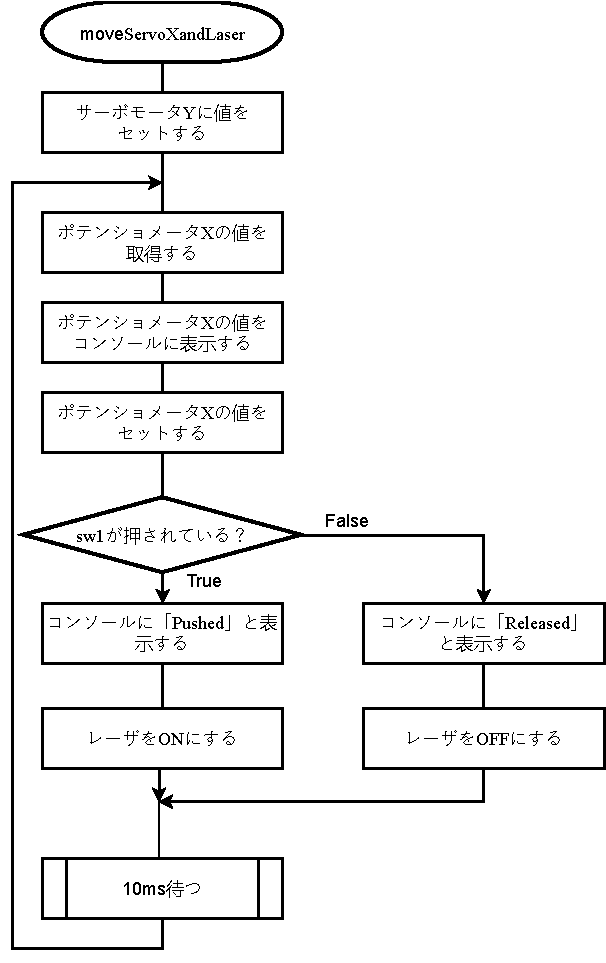
\includegraphics{kumikomi_flow_2.pdf}
    \caption{課題2フロウチャート}
    \label{fig:my_label}
\end{figure}

\subsection{実験方法}
サーボモータに値をセットし、sw1に変化が生じた時にイベントが発生するプログラムServoXandLaserを作成し、実行した.

\begin{lstlisting}[caption=ServoXandLaser]

import hardware.*;
//import stub.*;
public class Kadai2_ServoXandLaser
{
    private Hardware hardware = Hardware.getInstance();//ハードウェアのインスタンスを取得する

    public void moveServoXandLaser() {
        hardware.drawUnit.servoY.setValue(5);
        //サーボモータYにとりあえずの値をおいておく サーボモータYが描画領域にないとだめなので適宜調整
        while(true){
            int potXvalue = hardware.manipulator.potX.getValue();
            //ポテンションメーターxの値を取得する
            System.out.print("PotX = " + potXvalue);//potXの値を表示
            hardware.drawUnit.servoX.setValue(potXvalue);//サーボモータXniatai をセットする
            System.out.print("       ");
            System.out.print("SW1 = ");
            if (hardware.manipulator.sw1.isPush()){//sw1が押されているかを判定
                System.out.print("Pushed");//押されていたら「pushed」と表示
                hardware.drawUnit.laser.on();//レーサをonにする
            }else{
                System.out.print("Relesed");//押されていなければ「Relesed」と表示
                hardware.drawUnit.laser.off();//レーザをoffにする
            }
            System.out.println();//改行する
            wait_ms(10);//10ms待つ(サーボモータの使用上)
        }
    }

    private void wait_ms( int waitTime_ms) {//ms単位で指定するウェイトメソット
        try {
            Thread.sleep(waitTime_ms);

        } catch (Exception e) {
            //nothing to do (この課題では関係ない)
        }
    }
}
\end{lstlisting}

\subsection{結果}
ああ
\begin{table}[h]
    \centering
    \begin{tabular}{c|c|c}
      スイッチ1の状態   & ポテンションメータXの状態 &結果 \\
\hline\hline
        押さない & 右から左に回し切った &
        \begin{tabular}{c}
            レーザ光は光らず、\\potX=0からpot=255まで増加した  \\
        \end{tabular}
        \\
        
        \hline
        押さない & 右から左に回し切った &
        \begin{tabular}{c}
            レーザ光は光らず、\\potX=255からpot=0まで減少した  \\
        \end{tabular}
        \\
        \hline\hline
        押す& 回さない&
        \begin{tabular}{c}
            レーザ光が光り、\\sw1=Pushedと表示された  \\
        \end{tabular}
        \\
        \hline
        離す&回さない&
        \begin{tabular}{c}
            レーザ光は光らず、\\potX=255からpot=0まで減少した  \\
        \end{tabular}
        
        \\
        \hline
        
        押す&左端に回した&
        \begin{tabular}{c}
            描画範囲外になったため、レーザ光がどこにあるかわからなかった  \\
        \end{tabular}
        
        
    \end{tabular}
    \caption{Caption}
    \label{tab:my_label}
    
    
\end{table}

また、頻繁に用いられるウェイトルーチンをUnityToolsとして他のクラスからも使えるような形にした。
\begin{lstlisting}[caption=UtilityTools]
    public class UtilityTools
 {
 public static void wait_ms( int waitTime_ms ) {
 try {
 Thread.sleep( waitTime_ms );
 } catch ( Exception e ) {
 // nothing to do (この課題の用途では処理することがない)
 }
 }
 }
\end{lstlisting}

\subsection{考察}
sw1を押すことでのみレーザ光がONになっていることから、hardware.drawUnit.laser.on()によって
sw2やメータにより、レーザ光を制御ができると考えられた。


\section{課題3}
\subsection{目的}
ポテンションメータX,Yを用いてX軸、Y軸のサーボモータを動かして、レーザ光を自由に動かす。さらに
プッシュスイッチSW1を押したらレーザ光をON,
SWを押したらレーザ光をOFFにする。SW1、SW2を同時に押したらプログラムを終了させる。

\subsection{フロウチャート}

\begin{figure}[H]
    \centering
    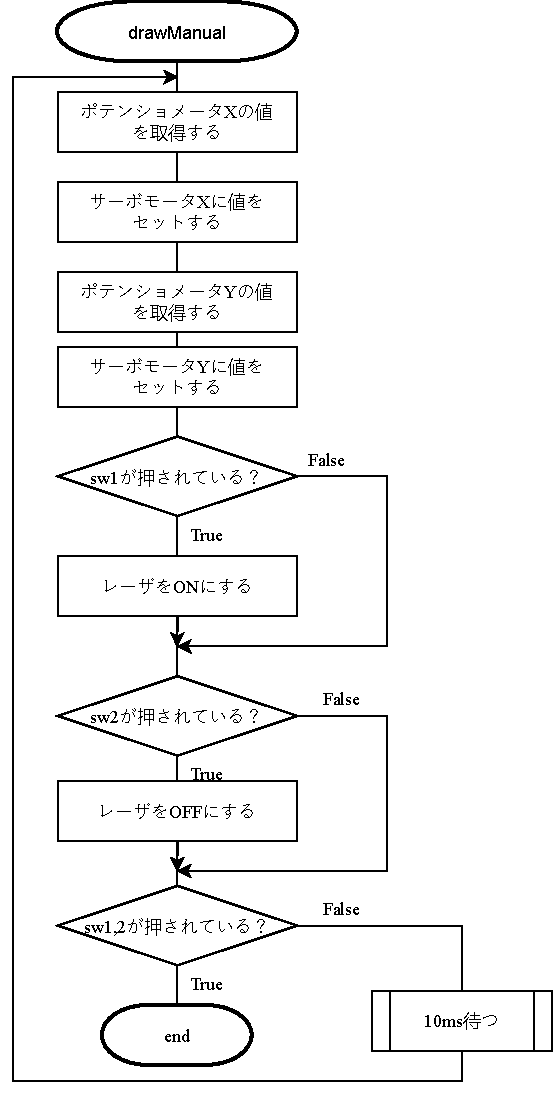
\includegraphics{kumikomi3.pdf}
    \caption{課題3のフロウチャート}
    \label{fig:my_label}
\end{figure}

\subsection{実験方法}

\begin{lstlisting}[caption=DrawManual]
import hardware.*;  //実験で実機を使用する場合にはコメントを外してこれを使用する
//import stub.*;  //予習などで実機を使用せずに動作を確認する場合には、これを使用する

public class Kadai3_DrawManual
{
    Hardware hardware = Hardware.getInstance(); //ハードウェアのインスタンスを取得する
    public void moveServoXandLaser() {
        System.out.println( "Kadai 3 start!" );
        while ( true ) {  //無限に繰り返す
            int potXvalue = hardware.manipulator.potX.getValue();        //ポテンショメーターXの値を取得する
            hardware.drawUnit.servoX.setValue(potXvalue );         //サーボモーターXに値をセットする
            int potYvalue = hardware.manipulator.potY.getValue();                  //ポテンショメーターYの値を取得する
            hardware.drawUnit.servoY.setValue(potYvalue );      //サーボモーターYに値をセットする
            
            boolean sw1isPush = hardware.manipulator.sw1.isPush();
            boolean sw2isPush = hardware.manipulator.sw2.isPush();
            if (hardware.manipulator.sw1.isPush()) {    //sw1が押されているか調べる
                hardware.drawUnit.laser.on()  ;     //レーザーをonにする
            }
            if (hardware.manipulator.sw2.isPush()) {    //sw2が押されているか調べる
                hardware.drawUnit.laser.off();       //レーザーをoffにする
            }
            if ( hardware.manipulator.sw1.isPush() && hardware.manipulator.sw2.isPush() ) {    //sw1とsw2が押されているか調べる
                System.out.println( "Kadai 3 end!" );
                System.exit( 0 );
            }
            UtilityTools.wait_ms( 10 );        //10ms 待つ
        }
    }
}
\end{lstlisting}

\subsection{結果}
起動させるとコンソールにKadai 3 Start!と表示された。
課題1,2と異なりコンソールには、メータを動かす、スイッチを押す等の変化がない限り表示は更新されない。
sw1,2を同時に押すとコンソールにKadai 3 end! と表示され、newしていたクラスが閉じた。

\subsection{考察}

スイッチ1,2を同時に押すことでプログラムを終了することができたことから、データを同時に送ることができることが分かった。

\section{課題4}
\subsection{目的}
 マニピュレーターの ポテンショメーター X または プッシュスイッチ SW1 の値が変化した ときのみ、その値を読み取り、コンソールに表示させる。

\subsection{フロウチャート}

\begin{figure}[H]
    \centering
    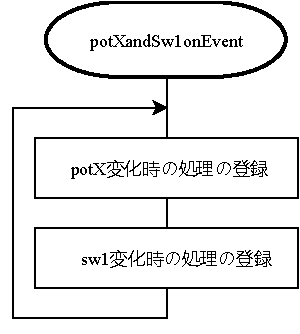
\includegraphics{kumikomi4.pdf}
    \caption{課題4の全体のフロウチャート}
    \label{fig:my_label}
\end{figure}

\begin{figure}[H]
    \centering
    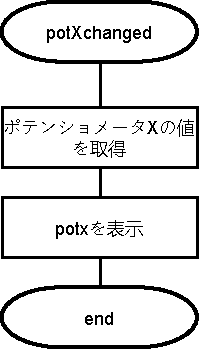
\includegraphics{kumikomi4potXchenged.pdf}
    \caption{potXが変化時の処理}
    \label{fig:my_label}
\end{figure}

\begin{figure}[H]
    \centering
    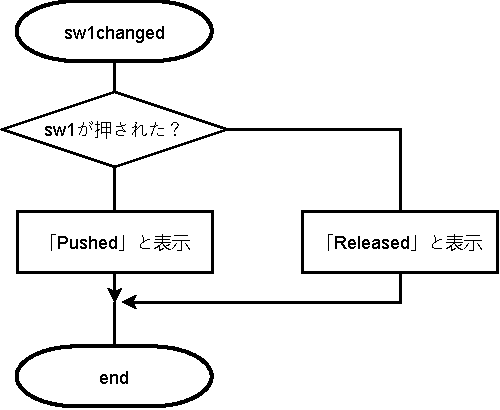
\includegraphics{kumikomi4se1changed.pdf}
    \caption{sw1が変化時の処理}
    \label{fig:my_label}
\end{figure}


\subsection{実験方法}

\begin{lstlisting}[caption=PotXandSw1]
import hardware.*;  //実験で実機を使用する場合にはコメントを外してこれを使用する
//import stub.*;  //予習などで実機を使用せずに動作を確認する場合には、これを使用する

public class Kadai4_PotXandSw1onEvent
{
    private Hardware hardware = Hardware.getInstance(); //ハードウェアのインスタンスを取得する

    public void dispPotXandSw1() {
        hardware.manipulator.potX.addListener( () ->potXchanged()  );  //potXが変化したときに処理したいメソッド
        hardware.manipulator.sw1.addListener( () ->sw1changed() );  //sw1が変化したときに処理したいメソッド

        while ( true ) {  //無限に繰り返す
            // nothing to do  (この課題の用途では処理することがない)
        }
    }

    // ポテンショメータX変化時の処理メソッド
    private void potXchanged() {
        int potXvalue = hardware.manipulator.potX.getValue();   
        //ポテンショメーターXの値を取得する
        System.out.println( "PotX = " + potXvalue );    //potXの値を表示する
    }

    // プッシュスイッチSW1変化時の処理メソッド
    private void sw1changed() {
        System.out.print( "SW1 = " );
        if ( hardware. manipulator.sw1.isPush() ) { //sw1が押されているか調べる
            System.out.println( "Pushed" );  //押されていたら「Pushed」と表示する
        } else {
            System.out.println( "Released" ); //押されてなければ「Released」と表示する
        }
    } 
}
\end{lstlisting}

\subsection{結果}
\begin{table}[h]
    \centering
    \caption{課題4}
    \begin{tabular}{c|c}
    やったこと&コンソールの表示\\
    \hline\hline
    
    メータを左端で止めておく     &  何も表示されない\\
    \hline
    メータを右に動かす     & potX= の値が段々と増加する\\
    \hline
    右に回し切った & potX=255の表示で止まった\\
    \hline
    メータを左端にし、sw1を押した&sw1=Pushed
    \hline
    sw1を離した&sw1=Released
    \hline
    sw1を1秒間押し続けた&sw1=Pushedを一回のみ表示した
    \end{tabular}
    
    \label{tab:my_label}
\end{table}


\subsection{考察}
課題1の時とは異なり、コンソールの表示が常に更新されるのではなく、変化が生じた時の表示された
ことより、
イベントドリブンを用いると、変化が生じたときにのみ実行できることが分かった。

また、これを用いることでイベントが起きていないときのメモリの負荷を減らすことができていると考えられる。

\section{課題5}
\subsection{目的}
 レーザー光を on にしておき、ポテンショメーターX , Y を使って X 軸用と Y 軸用のサーボモ ーターを動かして、レーザー光を自由に動かす。
また、プッシュスイッチ SW1 を押したらサーボモーターX , Y への指示値をコンソールに表 示してください。
さらに、SW2 が押されたら、プログラムを終了させる。

\subsection{フロウチャート}

\begin{figure}[H]
    \centering
    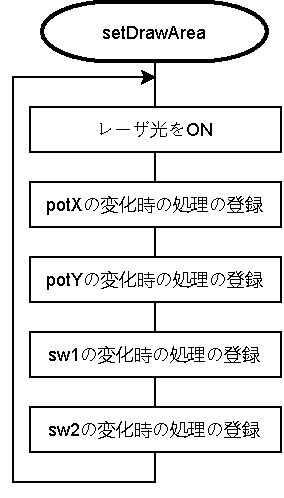
\includegraphics{kadai5setDrawArea-Page-1.pdf}
    \caption{setDrawAreaの全体のフロウチャート}
    \label{fig:my_label}
\end{figure}

\begin{figure}[H]
    \centering
    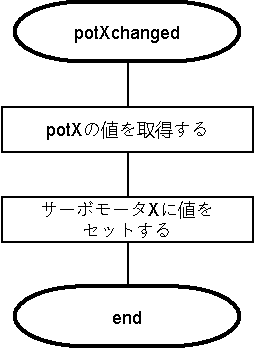
\includegraphics{kadai5setDrawArea-potXchanged.pdf}
    \caption{potXの変化時の処理}
    \label{fig:my_label}
\end{figure}

\begin{figure}[H]
    \centering
    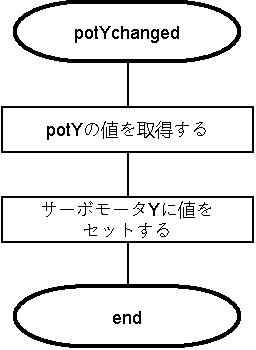
\includegraphics{kadai5setDrawArea-potY.pdf}
    \caption{potYの変化時の処理}
    \label{fig:my_label}
\end{figure}

\begin{figure}[H]
    \centering
    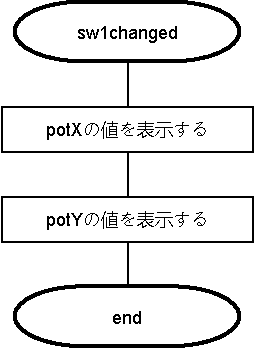
\includegraphics{kadai5setDrawArea-sw1.pdf}
    \caption{sw1変化時の処理}
    \label{fig:my_label}
\end{figure}

\begin{figure}[H]
    \centering
    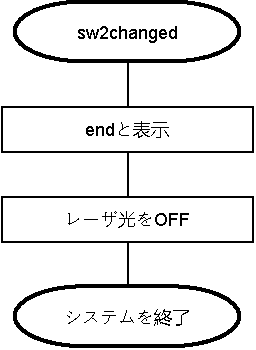
\includegraphics{kadai5setDrawArea-sw2.pdf}
    \caption{sw2の変化時の処理}
    \label{fig:my_label}
\end{figure}


\subsection{実験方法}

\begin{lstlisting}[caption=SetDrawArea]
import hardware.*; //実験で実機を使用する場合にはコメントを外してこれを使用する
//  import stub.*; //予習などで実機を使用せずに動作を確認する場合には、これを使用する
public class Kadai5_SetDrawArea
{
    // インスタンス変数 - コードに合わせて説明を書き換えます.
    private Hardware hardware = Hardware.getInstance();//ハードウェアのインスタンスを取得する
    int potXvalue ; 
    int potYvalue ;
    
    public void SetDrawArea(){
    
        hardware.drawUnit.laser.on();
        
        hardware.manipulator.potX.addListener(()->potXchanged());
        hardware.manipulator.potY.addListener(()->potYchanged());
        hardware.manipulator.sw1.addListener(()->sw1changed());
        hardware.manipulator.sw2.addListener(()->sw2changed());
        while ( true ) {  //無限に繰り返す
            // nothing to do  (この課題の用途では処理することがない)
        }
    }
    
    private void potXchanged(){//potXを変えたら変数に格納
        potXvalue = hardware.manipulator.potX.getValue();
        hardware.drawUnit.servoX.setValueUnlimited(potXvalue );         //サーボモーターXに値をセットする
    }
    private void potYchanged(){//potYを変えたら...
        potYvalue = hardware.manipulator.potY.getValue();
        hardware.drawUnit.servoY.setValueUnlimited(potYvalue );      //サーボモーターYに値をセットする
    }
    private void sw1changed(){//sw1を押したときに呼び出し
        System.out.print("potX= "+potXvalue);
        System.out.println(" ,potY= "+potYvalue);
    }
    private void sw2changed(){//sw2を押したら..
        System.out.println("End!");
        hardware.drawUnit.laser.off();
        System.exit(0);
        
    }
}
    

\end{lstlisting}

\subsection{結果}
\\


\begin{table}[h]
    \centering
    \caption{課題5}
    \begin{tabular}{c|c}
    使用機材の番号     &DXY-150  \\
    \hline
    左の限界値     &119\\
    右の限界値  &213\\
    手前の限界値&29\\
    奥の限界値&140\\
    \end{tabular}
    
    \label{tab:my_label}
\end{table}

sw2を押すとコンソールにEnd!と表示され、プログラムが終了した。
\subsection{考察}

レーザ光が斜めに動くために描画領域は想定していたものより小さくなった。

\section{課題6}

\subsection{目的}
 描画領域の限界値(サーボモーターの可動有効範囲)を設定し、設定した限界値で描画領域 をはみ出すことがないか、図形を描いて確認する。


\subsection{フロウチャート}

\begin{figure}[H]
    \centering
    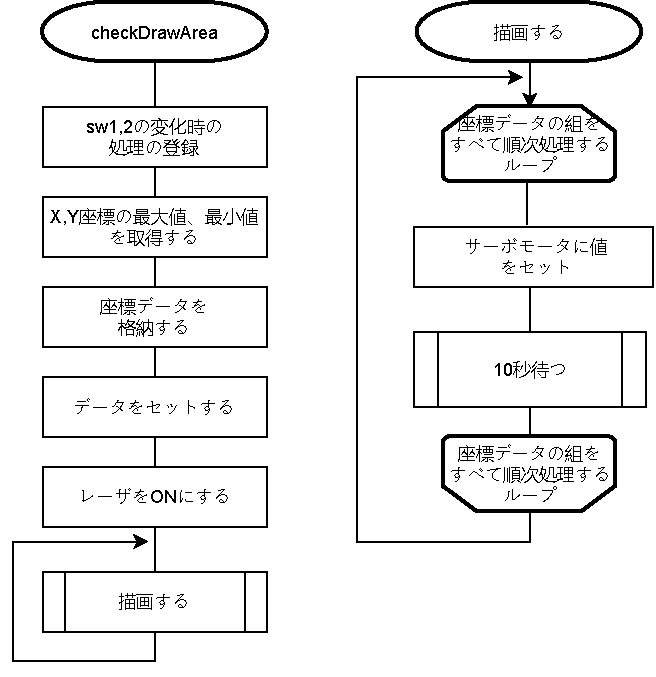
\includegraphics{kumikomi6-checkDrawArea.pdf}
    \caption{checkDraeAreaの全体のフロウチャート}
    \label{fig:my_label}
\end{figure}

\begin{figure}[H]
    \centering
    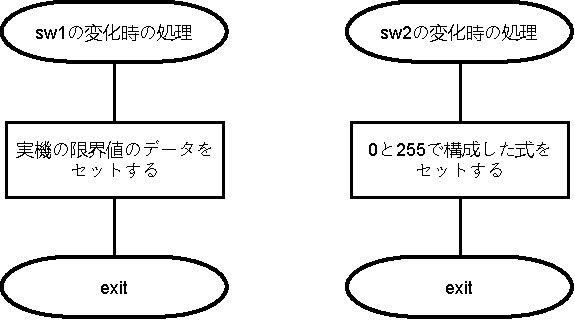
\includegraphics{kumikomi6-swChenged.pdf}
    \caption{各イベントのフロウチャート}
    \label{fig:my_label}
\end{figure}


\subsection{実験方法}

\begin{lstlisting}[caption=CheckDrawArea]
 import hardware.*;  //実験で実機を使用する場合にはコメントを外してこれを使用する
//import stub.*;  //予習などで実機を使用せずに動作を確認する場合には、これを使用する

public class Kadai6_CheckDrawArea
{
    private Hardware hardware = Hardware.getInstance(); //ハードウェアのインスタンスを取得する
    private int[] xA = new int[8];  //getMin(),getMax()での座標データ配列
    private int[] yA = new int[8];  //getMin(),getMax()での座標データ配列

    //                   左下 左上 右上 右下  左下 右上 左上 右下
    private int[] xB = {   0,   0,  255,  255, 0,  255,  0, 255 };
    private int[] yB = {    0 ,   255, 255, 0, 0,  255,   255, 0 };

    private int[] drawX;  //描画用データ配列(X座標)
    private int[] drawY;  //描画用データ配列(Y座標)

    public void checkDrawArea() {
        hardware.manipulator.sw1.addListener( () -> selectDataA() );
        hardware.manipulator.sw2.addListener( () -> selectDataB() );

        hardware.drawUnit.servoX.setMinMax(    119,213    ); //X座標の最小値と最大値を入れる
        hardware.drawUnit.servoY.setMinMax(    29,140    ); //Y座標の最小値と最大値を入れる

        int xMin = hardware.drawUnit.servoX.getMin(); //X座標の最小値を取得する
        int xMax = hardware.drawUnit.servoX.getMax(); //X座標の最大値を取得する
        int yMin = hardware.drawUnit.servoY.getMin(); //Y座標の最小値を取得する
        int yMax = hardware.drawUnit.servoY.getMax(); //Y座標の最大値を取得する

        xA[0] =   xMin   ; //左下        //座標データの格納
        yA[0] =  yMin  ; 
        xA[1] =  xMin ; //左上
        yA[1] =  yMax ;
        xA[2] =  xMax  ; //右上
        yA[2] =  yMax  ;
        xA[3] =  xMax ; //右下
        yA[3] =  yMin  ;
        xA[4] =  xMin  ; //左下
        yA[4] =  yMin  ; 
        xA[5] =  xMax ; //右上
        yA[5] =  yMax ;
        xA[6] =   xMin  ; //左上
        yA[6] =   yMax  ;
        xA[7] =   xMax ; //右下
        yA[7] =   yMin ;

        selectDataA();  // 描画するデータにxA[],yA[]を選択する
        hardware.drawUnit.laser.on();
        while ( true ) {
            for ( int i=0 ; i<drawX.length ; i++ ) {
                hardware.drawUnit.servoX.setValue( drawX[i] );
                hardware.drawUnit.servoY.setValue( drawY[i] );
                UtilityTools.wait_ms( 100 );
            }
        }
    }

    private void selectDataA() {
        drawX = xA;
        drawY = yA;
        hardware.raspIfBoard.setLed( 0x08 );
        for ( int i=0 ; i<drawX.length ; i++ ) {
            System.out.printf( "(%3d,%3d)" , drawX[i] , drawY[i] );
        }
        System.out.println();
    }

    private void selectDataB() {
        drawX = xB;
        drawY = yB;
        hardware.raspIfBoard.setLed( 0x01 );
        for ( int i=0 ; i<drawX.length ; i++ ) {
            System.out.printf( "(%3d,%3d)" , drawX[i] , drawY[i] );
        }
        System.out.println();
    }
}

\end{lstlisting}
\newpage
\subsection{結果}

\begin{figure}[h]
    \centering
    
    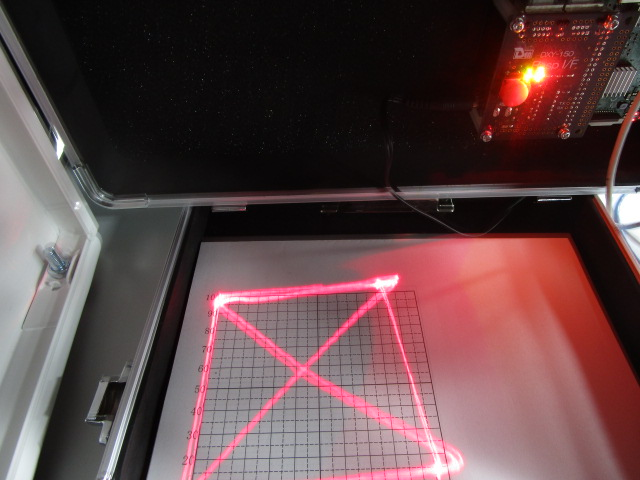
\includegraphics[width=5cm]{IMG_1736.JPG}
    \caption{課題6:sw1を押し、0と255で構成した式を実行したたとき}
    \label{fig:my_label}
\end{figure}

\begin{figure}[h]
    \centering
    
    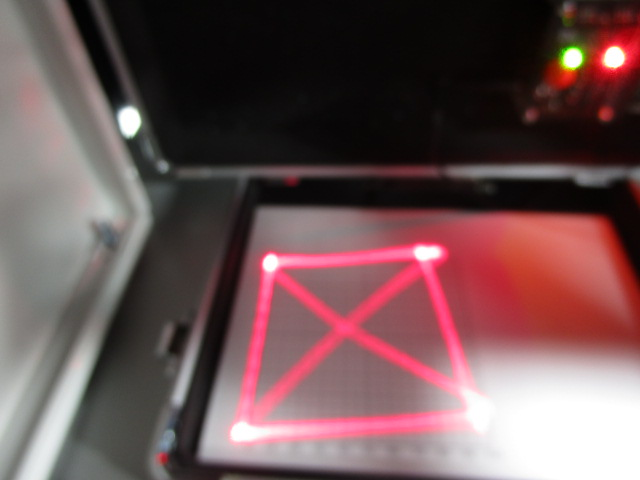
\includegraphics[width=5cm]{IMG_1737.JPG}
    \caption{課題6:sw2を押したとき}
    \label{fig:my_label}
\end{figure}


\subsection{考察}
0と255で構成された式で描いた図形と限界値を設定した式で描いたものは同じになった。
また、LEDを用いることで何を実行しているかを判別することができることが分かった。

\section{課題7}
\subsection{目的}
 使用している機械が違っても、描画領域への座標指定の数値は同じ値で指定できるように、 共通化できる仕組みを実装する。
 共通化したデータの指定方法は、次のルールに従う。 「描画領域の左下の座標を(0,0)、右上の座標を(100,100)とし、内部は線形とする」


\subsection{フロウチャート}

\begin{figure}[H]
    \centering
    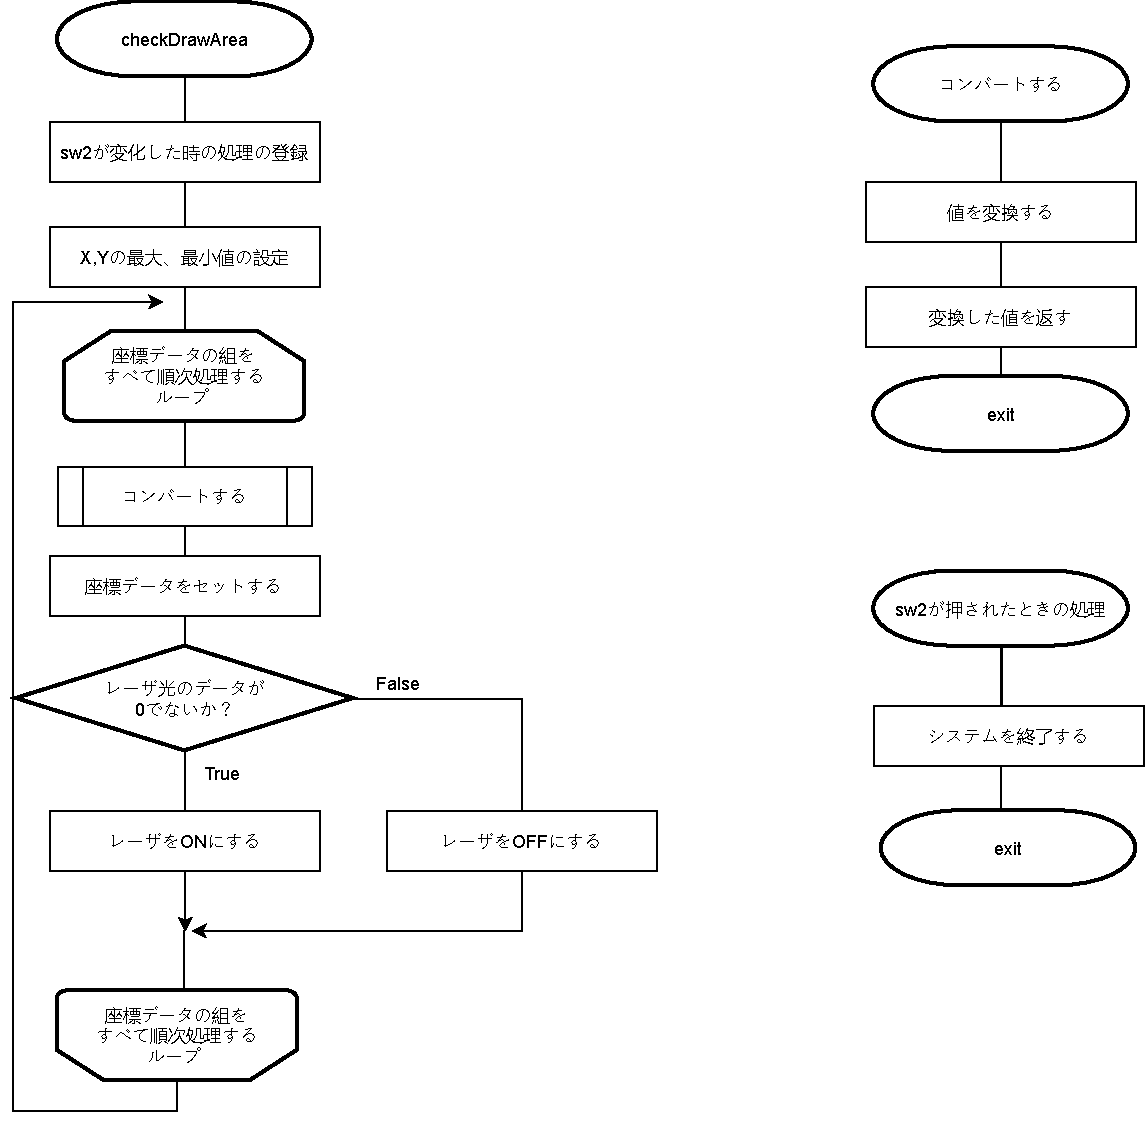
\includegraphics[scale=0.8]{kumikomiKadai7..pdf}
    \caption{課題7のフロウチャート}
    \label{fig:my_label}
\end{figure}


\subsection{実験方法}

\begin{lstlisting}[caption=CheckDrawArea2]
  import hardware.*;  //実験で実機を使用する場合にはコメントを外してこれを使用する
//import stub.*;  //予習などで実機を使用せずに動作を確認する場合には、これを使用する

public class Kadai7_CheckDrawArea2
{
    private Hardware hardware = Hardware.getInstance(); //ハードウェアのインスタンスを取得する

    public void checkDrawArea() {
        System.out.println( "Kadai 7 Start!" );
        hardware.manipulator.sw2.addListener( () -> systemExit() );

        hardware.drawUnit.servoX.setMinMax(   119 , 213   ); //X座標の最小値と最大値を入れる
        hardware.drawUnit.servoY.setMinMax(  29  , 140   ); //Y座標の最小値と最大値を入れる

        while ( true ) {
            for ( int[] point : Figure.drawAreaCheck ) {
                hardware.drawUnit.servoX.setValue( convertX( point[Figure.X] ) );
                hardware.drawUnit.servoY.setValue( convertY( point[Figure.Y] ) );
                if ( point[Figure.LASER] == Figure.ON ) {
                    hardware.drawUnit.laser.on();
                } else {
                    hardware.drawUnit.laser.off();
                }
                System.out.println( "(" + point[Figure.X] + "," + point[Figure.Y] + ")" );
                UtilityTools.wait_ms( 100 );
            }
        }
    }

    private int convertX( int x ) {
        int xMin = hardware.drawUnit.servoX.getMin();
        int xMax = hardware.drawUnit.servoX.getMax();
        double X = x*(xMax-xMin)/100+xMin;
        return ( (int)X );  //この部1
    }
        
    private int convertY( int y ) {
        int yMin = hardware.drawUnit.servoY.getMin();
        int yMax = hardware.drawUnit.servoY.getMax();
        double Y = y*(yMax-yMin)/100+yMin ;
        return ( (int)Y );  //この部分に変換式を記述する
    }

    private void systemExit() {
        hardware.reset();
        System.out.println( "Kadai 7 End." );
        System.exit( 0 );
    }
}
\end{lstlisting}

また、描画する図形データををクラス名figureに
まとめる。

\begin{lstlisting}[caption=figure]
   public class Figure
{
    public static final int X = 0;       // X座標データのインデックス
    public static final int Y = 1;       // Y座標データのインデックス
    public static final int LASER = 2;   // レーザーON/OFFデータのインデックス
    public static final int ON = 1;   //「ON」の定数定義
    public static final int OFF = 0;  //「OFF」の定数定義
    
    static int[][] drawAreaCheck = {    //描画領域を確認する「☒型」のデータ
        {   0,   0, ON  } ,  //左下
        {   0, 100, ON  } ,  //左上
        { 100, 100, ON  } ,  //右上
        { 100,   0, ON  } ,  //右下
        {   0,   0, ON  } ,  //左下
        { 100, 100, ON  } ,  //右上
        {   0, 100, ON  } ,  //左上
        { 100,   0, ON  } ,  //右下
    };
}
\end{lstlisting}

\subsection{結果}
\begin{figure}[h]
    \centering
    
    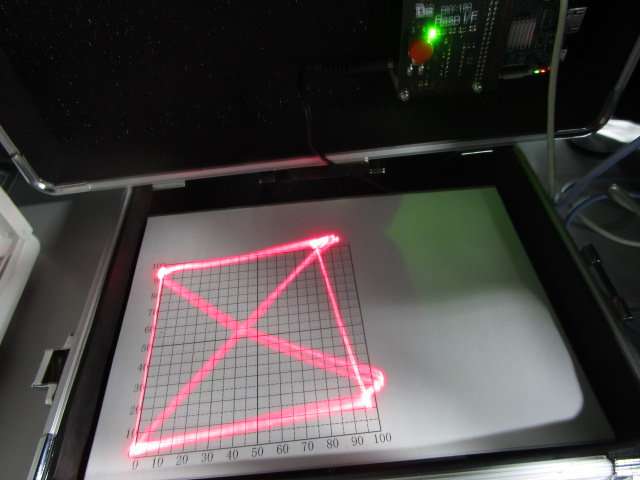
\includegraphics[width=5cm]{IMG_1738.JPG}
    \caption{課題7}
    \label{fig:my_label}
\end{figure}


\subsection{考察}


正規化された値を実機の値に変換する式は
$$実機の値 = A×(入力された、正規化された値) + B $$
である。この式に、(実機の値=Min,入力する値=0)、(実機の値=Max,入力する値=
100)を代入する。


 
\begin{numcases}
{}
Min&=A×0+B \\
Max&=A×100+B
\end{numcases}



(1)よりB=Min\\
これを(2)に代入し\\
Max=A×100+Min\\
100×A=Max-Min\\
A=$\frac{Max-Min}{100}$ \\
したがって、正規化した値を実機の値に直す
式は、
\begin{equation}
実機に入力する値=\frac{Max-Min}{100}×入力された値+Min
\end{equation}

また、課題6と同様の図形が描画できたため、convertの式が正しいと考えられる。
\newpage

\section{課題8}
\subsection{目的}
 描かせたい図形を描画領域上でトレースして頂点情報をプロットし、図形データを作成する ツールを作成する。
 また、作成した図形データを確認するツールも併せて作成する。


\subsection{フロウチャート}

\begin{figure}[H]
    \centering
    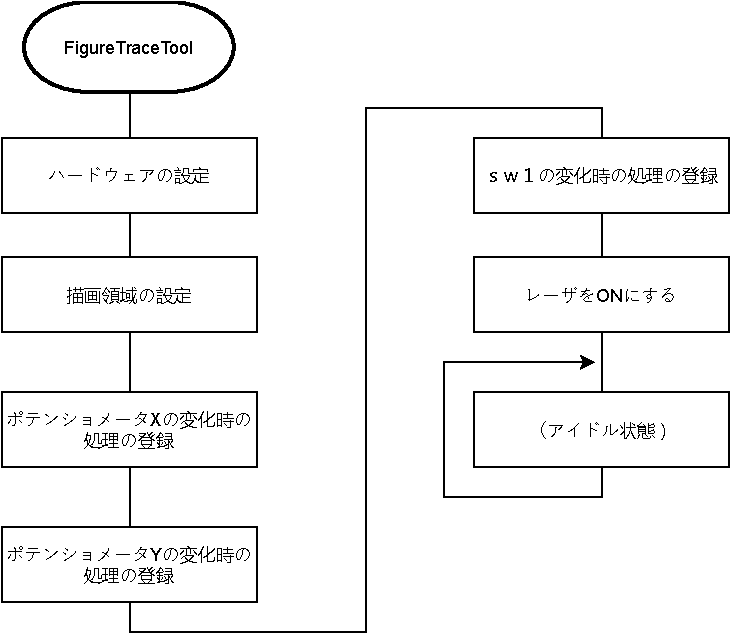
\includegraphics{kumikomiKadai8figureTraceTool.pdf}
    \caption{FigureTraceToolのイベントのフロウチャート}
    \label{fig:my_label}
\end{figure}

\begin{figure}[H]
    \centering
    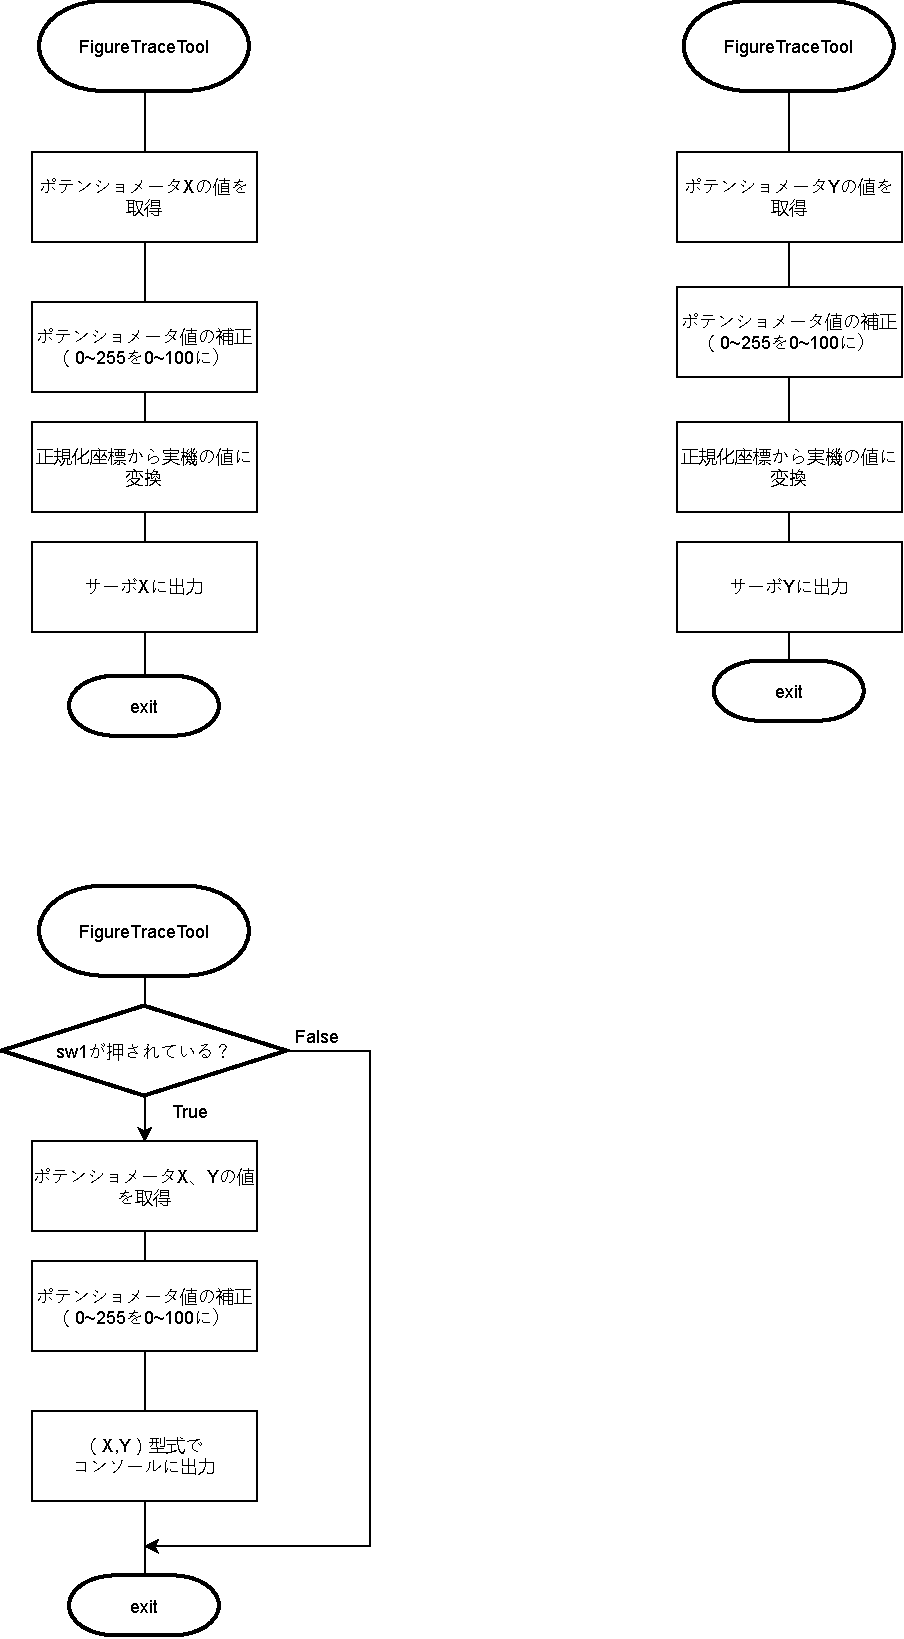
\includegraphics[scale=0.9]{kumikomiKadai8-event.pdf}
    \caption{FigureTraceToolのイベントのフロウチャート}
    \label{fig:my_label}
\end{figure}

\begin{figure}[H]
    \centering
    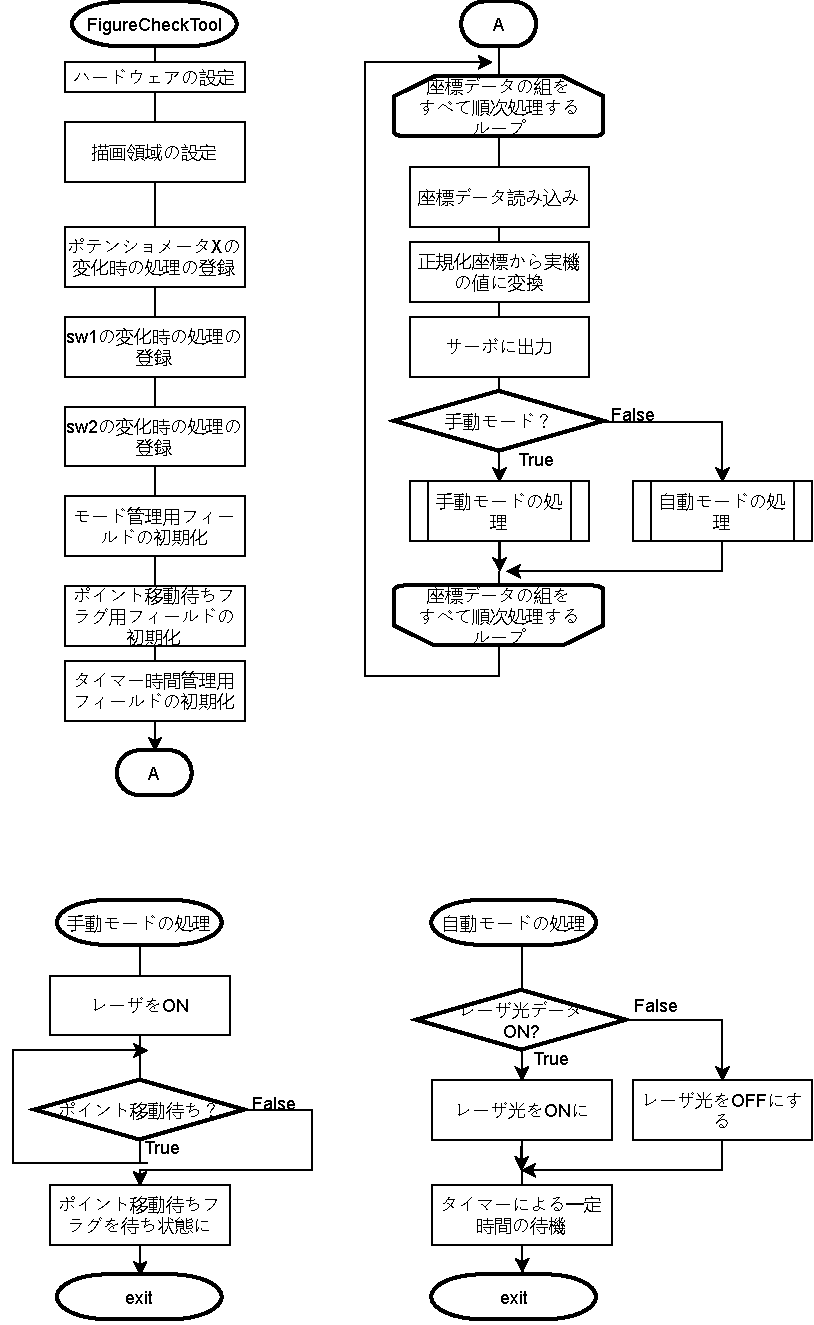
\includegraphics{kumikomiKadai8-FigureCheckTolAll.pdf}
    \caption{FigureCheckToolの全体のフロウチャート}
    \label{fig:my_label}
\end{figure}

\begin{figure}[H]
    \centering
    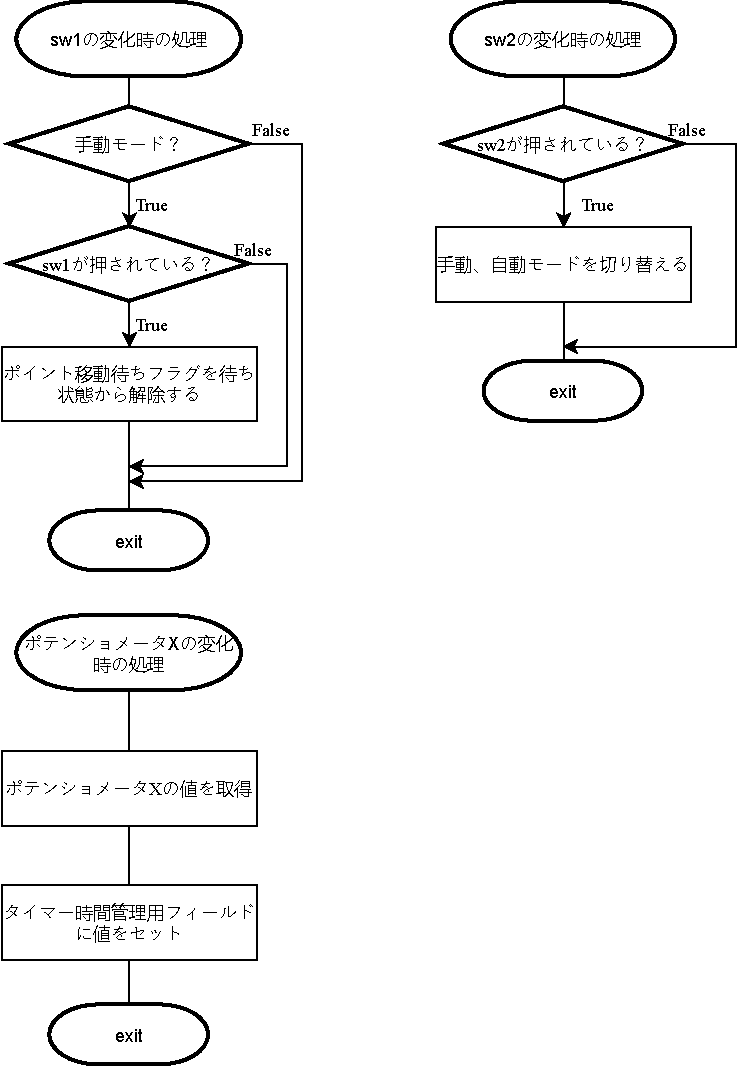
\includegraphics{kumikomiKadai8-figureCheckToolEvent.pdf}
    \caption{FigureCheckToolのイベントのフロウチャート}
    \label{fig:my_label}
\end{figure}

\subsection{実験方法}

必要になる機能を表に並べた
。


\begin{table}[h]
    \caption{表8-1 図形データ作成ツールの機能}
    \centering
    \begin{tabular}{|c|c|c|}
    \hline
    \rowcolor[rgb]{0.9,0.9,0.9}
    項目番号&機能&説明\\
    \hline
     1    &図形のトレース &描画領域上で紙に描かれた図形をなぞれるようにする \\
     \hline
      2   & 頂点のプロット&図形の頂点に当たるところの座標を表示・登録する\\
       \hline  
     3  &データの確認  & 作成したデータに問題が無いか確認できるようにする\\
       \hline
    
       
    \end{tabular}
    \caption{Caption}
    \label{tab:my_label}
\end{table}



\begin{table}[h]
    \caption{表8-2 使用機材の機能や環境}
    \centering
    \begin{tabular}{|c|c|c|}
    \hline
    \rowcolor[rgb]{0.9,0.9,0.9}
    項目番号&機能&説明\\
    \hline
    \rowcolor[rgb]{0.8,0.8,0.8}
     1    & 操作系 &  自由な用途で使用できる操作系は以下の通り\\
     \hline
       1-1  & アナログ入力&回転型テンションメータが2系統\par 
       (入力値は実数、左回し切りの時が0)\\
       \hline  
       1-2&スイッチ入力   &モーメンタリーの押しボタンスイッチが 2 系統   (押している間だけ ON) \\
       \hline
       \rowcolor[rgb]{0.8,0.8,0.8}
       2 & 出力系&自由な用途で使用できる出力は以下の通り \\
        \hline
       2-1&レーザ光&縦横 2 軸で位置決めできる。座標指定は0~100 On/Off 可能 \\
       \hline
       
       2-2&LED&
       
       \begin{tabular}{c}
         赤色 4個。横 1 列等間隔で配置されている。\\ 独立して点灯/消灯できる
       \end{tabular}
        \\ \hline
        
        \rowcolor[rgb]{0.8,0.8,0.8}
        3&表示&情報の表示は以下の通り
        \\ \hline
        3-1&コンソール画面&文字の配置に自由度はなく、改行のみ
        \\
        \hline
        
        
    \end{tabular}
    
    \label{tab:my_label}
\end{table}



\begin{table}[h]
    \caption{表8-3 全体の構成}
    \centering
    \begin{tabular}{|c|c|c|}
    \hline
    \rowcolor[rgb]{0.9,0.9,0.9}
    項目番号&機能&説明\\
    \hline
    \rowcolor[rgb]{0.8,0.8,0.8}
     1    & ツールの構成&
     \begin{tabular}{c}
操作系や表示の煩雑さをなくすため、\\独立した 2 つのツ ールに分ける。 
     \end{tabular}
     \\
     \hline

       1-1  &データ作成ツール &
       
       \begin{tabular}{c}
            レーザー光のポインタを手動で移動させ、\\目的の位置で ボタンを押すと座標が表示されるようにする。
       \end{tabular}
       \\
       \hline  
       1-2&データ確認ツール   &
       
       \begin{tabular}{c}
        作成済みのデータの座標情報をボタンを押すごとに順次\\ 読み出し、移動したレーザー光の位置を確認する
       \end{tabular}
       
       \\
       \hline
    \end{tabular}

    \label{tab:my_label}
\end{table}

\newpage

\begin{table}[h]
    \caption{表8-4 各機能の対応や割り当て}
    \centering
    \begin{tabular}{|c|c|c|}
    \hline
    \rowcolor[rgb]{0.9,0.9,0.9}
    項目番号&機能&説明\\
    \hline
    
    \rowcolor[rgb]{0.8,0.8,0.8}
     1&
     データ作成ツール  &
     \begin{tabular}{c}
    レーザー光のポインタを手動で移動させ、目的の位置で\\ ボタンを押すと座標が表示されるようにする。
     \end{tabular}
      \\
    \hline
    1-1 &ポインタの移動 &
    \begin{tabular}{c}
    2つあるポテンショメーターを x 軸用とy軸用にする
    \end{tabular}
    
    \\
    \hline
    
    1-2&座標の登録
    &
    \begin{tabular}{c}
    目的の位置でボタンを押すことにより、コンソールに座 標を表示する。\\
    自動登録はデータの挿入や削除など、デ ータ編集部分での\\処理が多くなるので、今回は見送る。\\ 表示された座標を登録者が順序や妥当性を判断し、
    \\
    手書 きでデータを作成したのち、電子化する。
         
    \end{tabular}
 \\
 \hline
 
 \rowcolor[rgb]{0.8,0.8,0.8}
     2&
     データ確認ツール  &
     \begin{tabular}{c}
    作成済みのデータの座標情報をボタンを押すごとに順次\\ 読み出し、移動したレーザー光の位置を確認する。
     \end{tabular}
      \\
    \hline
 
 2-1
 & ポインタの移動&
 \begin{tabular}{c}
  描画範囲の座標は0~100なので、ポテンショメータ\\ の最小値が0、最大値が 100 となるようにする
 \end{tabular}
 \\
 \hline
 
 
 2-2&登録座標の読み取り&
 \begin{tabular}{c}
手動送りと自動送りのモードを設け、SW2\\ でモードを 切り替える。\\
手動送りの場合は、SW1 で登録ポイントを送る。\\ 自動送りの場合は、登録ポイントを自動的に送る。送り \\時間の間隔はポテンショメータ X で調整する。
 \end{tabular}
 \\
 \hline

    \end{tabular}
\end{table}

\begin{table}[]
    \centering
    \caption{8-5 各機能の詳細}
    \begin{tabular}{|c|c|c|}
    \hline
    \rowcolor[rgb]{0.9,0.9,0.9}
    項目番号&機能&説明\\
    \hline
    \rowcolor[rgb]{0.8,0.8,0.8}
     1&
     データ作成ツール  &
     \begin{tabular}{c}
    FigureTraceTool とする。 \\
    レーザー光は常に ON とする。
     \end{tabular}
     \\
     \hline
     
     1-1&ポインタの移動&
     \begin{tabular}{c}
    描画範囲の座標は0~100なので、ポテンショメータ \\の最小値が0、最大値が 100 となるようにする
     \end{tabular}
     \\
     \hline
     
     1-2& 座標の登録&
     \begin{tabular}{c}
    SW1 を押したら、その時点の座標を(x,y)の形式でコン\\ ソール表示する。
          
     \end{tabular}
     
     \\
     \hline
     \rowcolor[rgb]{0.8,0.8,0.8}
     2&データ確認ツール&
     \begin{tabular}{c}
    FigureCheckToolとする
     \end{tabular}
     \\
     \hline
     
     2-1&ポインタの移動&
     \begin{tabular}{c}
    レーザー光は、手動送りモードの時は常に ON とし、自\\ 動送りモードの時は、登録情報に従って ON/OFF す \\る。
     \end{tabular}
     \\
     \hline
     2-2&登録座標の読み取り&
     \begin{tabular}{c}
    SW2 を押すごとに手動送りと自動送りのモードを切り \\替える。\\
手動送りの場合は、SW1 で登録ポイントを送る。\\ 自動送りの場合は、登録ポイントを自動的に送る。送り \\時間の間隔はポテンショメータ X で調整する。
     \end{tabular}
     \\
     \hline
    \end{tabular}
    
    \label{tab:my_label}
\end{table}

\newpage

\begin{lstlisting}[caption=FigureCheckTool]
  import hardware.*; //実験で実機を使用する場合にはコメントを外してこれを使用する
//import stub.*; //予習などで実機を使用せずに動作を確認する場合には、これを使用する
public class Kadai8_FigureCheckTool{   
    private Hardware hardware = Hardware . getInstance () ; //ハードウェアのインスタンスを取得する
    public void checkDrawArea () {
        hardware . manipulator . sw2 . addListener ( () -> systemExit () );

        hardware . manipulator . potX . addListener ( () -> potXchanged () ) ;
        hardware . manipulator . sw1 . addListener ( () -> sw1changed () );
        hardware . manipulator . potY . addListener ( () -> potYchanged () ) ;

        hardware . drawUnit . servoX . setMinMax ( 119 ,213 ) ; //座標の最小値と最大値を入れるX
        hardware . drawUnit . servoY . setMinMax ( 29 ,140 ) ; //座標の最小値と最大値を入れるY
        hardware . drawUnit . laser . on () ;

        while ( true ) {
            for ( int [] point : Figure .  ) {//書きたい座標の配列を指定する
                hardware . drawUnit . servoX . setValue ( convertX ( point [0] ) );
                hardware . drawUnit . servoY . setValue ( convertY ( point [1] ) );
                if ( point [2] != 0 ) {

                } else {
                    hardware . drawUnit . laser . off () ;
                }
                System . out . println ( "(" + point [0] + "," + point [1] + ")"
                );
                UtilityTools . wait_ms ( 100 );
            }
        }
    }
    volatile boolean modeManual ;
    volatile boolean pointMoveWaitFlag ;
    volatile int waitTimeValue ;
    private void potXchanged () {
        int potXvalue = hardware . manipulator . potX . getValue () ;//ポテンショメーターの値を取得するX
        System . out . println ( " PotX ␣=␣" + potXvalue ); //の値を表示するpotX
    }

    private void potYchanged () {
        int potYvalue = hardware . manipulator . potY . getValue () ;
        System . out . println ( " PotY ␣=␣" + potYvalue ); //の値を表示するpotX
    }

    private void sw1changed () {
        System . out . print ( " SW1 ␣=␣" );
        if ( hardware . manipulator . sw1 . isPush () ) { 
            System . out . println ( " PotX ␣=␣" );
            System . out . println ( " PotY ␣=␣" );
        } else if ( hardware . manipulator . sw2 . isPush () ){

        } else if ( hardware . manipulator . sw1 . isPush () && hardware . manipulator . sw2 . isPush
        () ) {
            System . out . print ( " End!" );
            System . exit (0) ;
        } else {

        }
    }

    private int convertX ( int x ) {
        int xMin = hardware . drawUnit . servoX . getMin () ;
        int xMax = hardware . drawUnit . servoX . getMax () ;
        return (  x * (xMax-xMin)/100 + xMin ); //この部分に変換式を記述する
    }

    private int convertY ( int y ) {
        int yMin = hardware . drawUnit . servoY . getMin () ;
        int yMax = hardware . drawUnit . servoY . getMax () ;
        return (y*(yMax-yMin) /100 +yMin) ; //この部分に変換式を記述する
    }

    private void systemExit () {
        System . out . println ( " End ." );
        System . exit ( 0 );
    }

}
\end{lstlisting}
\\
\begin{lstlisting}[caption=FigureTraceTool]
   import hardware.*;  //実験で実機を使用する場合にはコメントを外してこれを使用する
//import stub.*;  //予習などで実機を使用せずに動作を確認する場合には、これを使用する
public class Kadai8_FigureTraceTool
{
    // インスタンス変数 - コードに合わせて説明を書き換えます.
    
    private Hardware hardware = Hardware.getInstance(); //ハードウェアのインスタンスを取得する
    private int[] drawX;  //描画用データ配列(X座標)
    private int[] drawY;  //描画用データ配列(Y座標)
    int Xvalue ;
    int Yvalue ;
    double standardX ;
    double standardY ;
    double potXvalue ;
    double potYvalue ;
    public void FigureTraceTool(){
        hardware.drawUnit.servoX.setMinMax(    119,213    ); //X座標の最小値と最大値を入れる
        hardware.drawUnit.servoY.setMinMax(    29,140    ); //Y座標の最小値と最大値を入れる
        
        int xMin = hardware.drawUnit.servoX.getMin(); //X座標の最小値を取得する
        int xMax = hardware.drawUnit.servoX.getMax(); //X座標の最大値を取得する
        int yMin = hardware.drawUnit.servoY.getMin(); //Y座標の最小値を取得する
        int yMax = hardware.drawUnit.servoY.getMax(); //Y座標の最大値を取得する
        
        hardware.manipulator.potX.addListener(()->potXchanged());
        hardware.manipulator.potY.addListener(()->potYchanged());
        hardware.manipulator.sw1.addListener(()->sw1changed());
        
        
        hardware.drawUnit.laser.on();
    }


    private void potXchanged(){//potXを変えたら変数に格納
        int xMin = hardware.drawUnit.servoX.getMin(); //X座標の最小値を取得する
        int xMax = hardware.drawUnit.servoX.getMax(); //X座標の最大値を取得する
        
        Xvalue = hardware.manipulator.potX.getValue();
        standardX = Xvalue * 100/255 ;
        potXvalue = standardX*(xMax-xMin)/100+xMin ;
        
        hardware.drawUnit.servoX.setValueUnlimited((int)potXvalue );         //サーボモーターXに値をセットする
    }
    
    private void potYchanged(){//potYを変えたら...
        int yMin = hardware.drawUnit.servoY.getMin(); //Y座標の最小値を取得する
        int yMax = hardware.drawUnit.servoY.getMax(); //Y座標の最大値を取得する
        Yvalue = hardware.manipulator.potY.getValue();
        standardY = Yvalue * 100/255 ;
        potYvalue = standardY*(yMax-yMin)/100+yMin ;
        
        hardware.drawUnit.servoY.setValueUnlimited((int)potYvalue );      //サーボモーターYに値をセットする
    }
    
    private void sw1changed(){//sw1を押したときに呼び出し
        System.out.print("potX= "+standardX);
        System.out.println(" ,potY= "+standardY);
    }
    
}
\end{lstlisting}

描画する図形のデータは、figureに格納した。

\begin{lstlisting}[caption=Figure]

public class Figure
{
   static int[][]  hexagon = {
      {22, 16, ON},
      {22, 81, ON},
      {54, 92, ON},
      {88, 65, ON},
      {77, 15, ON},
      {44 ,7, ON},
    }; 
    static int[][] octagon = {
        {11, 0, ON},
        {22, 82, ON},
        {53, 94, ON},
        {80,70,ON},
        {90 ,33 ,ON},
        {69, 11, ON},
        {39, 4, ON},
        {13, 20, ON},
    };    
    
    static int [][]fivePointStar = {
        {48,82,ON},
        {27,10,ON},
        {95,45,ON},
        {11,56,ON},
        {74,12,ON},
        {48,82,ON},
    };
}
\end{lstlisting}
\\
\subsection{結果(六角形)}
描画させる図形の方眼紙の図は図21である。
\begin{figure}[H]
    \centering
    
    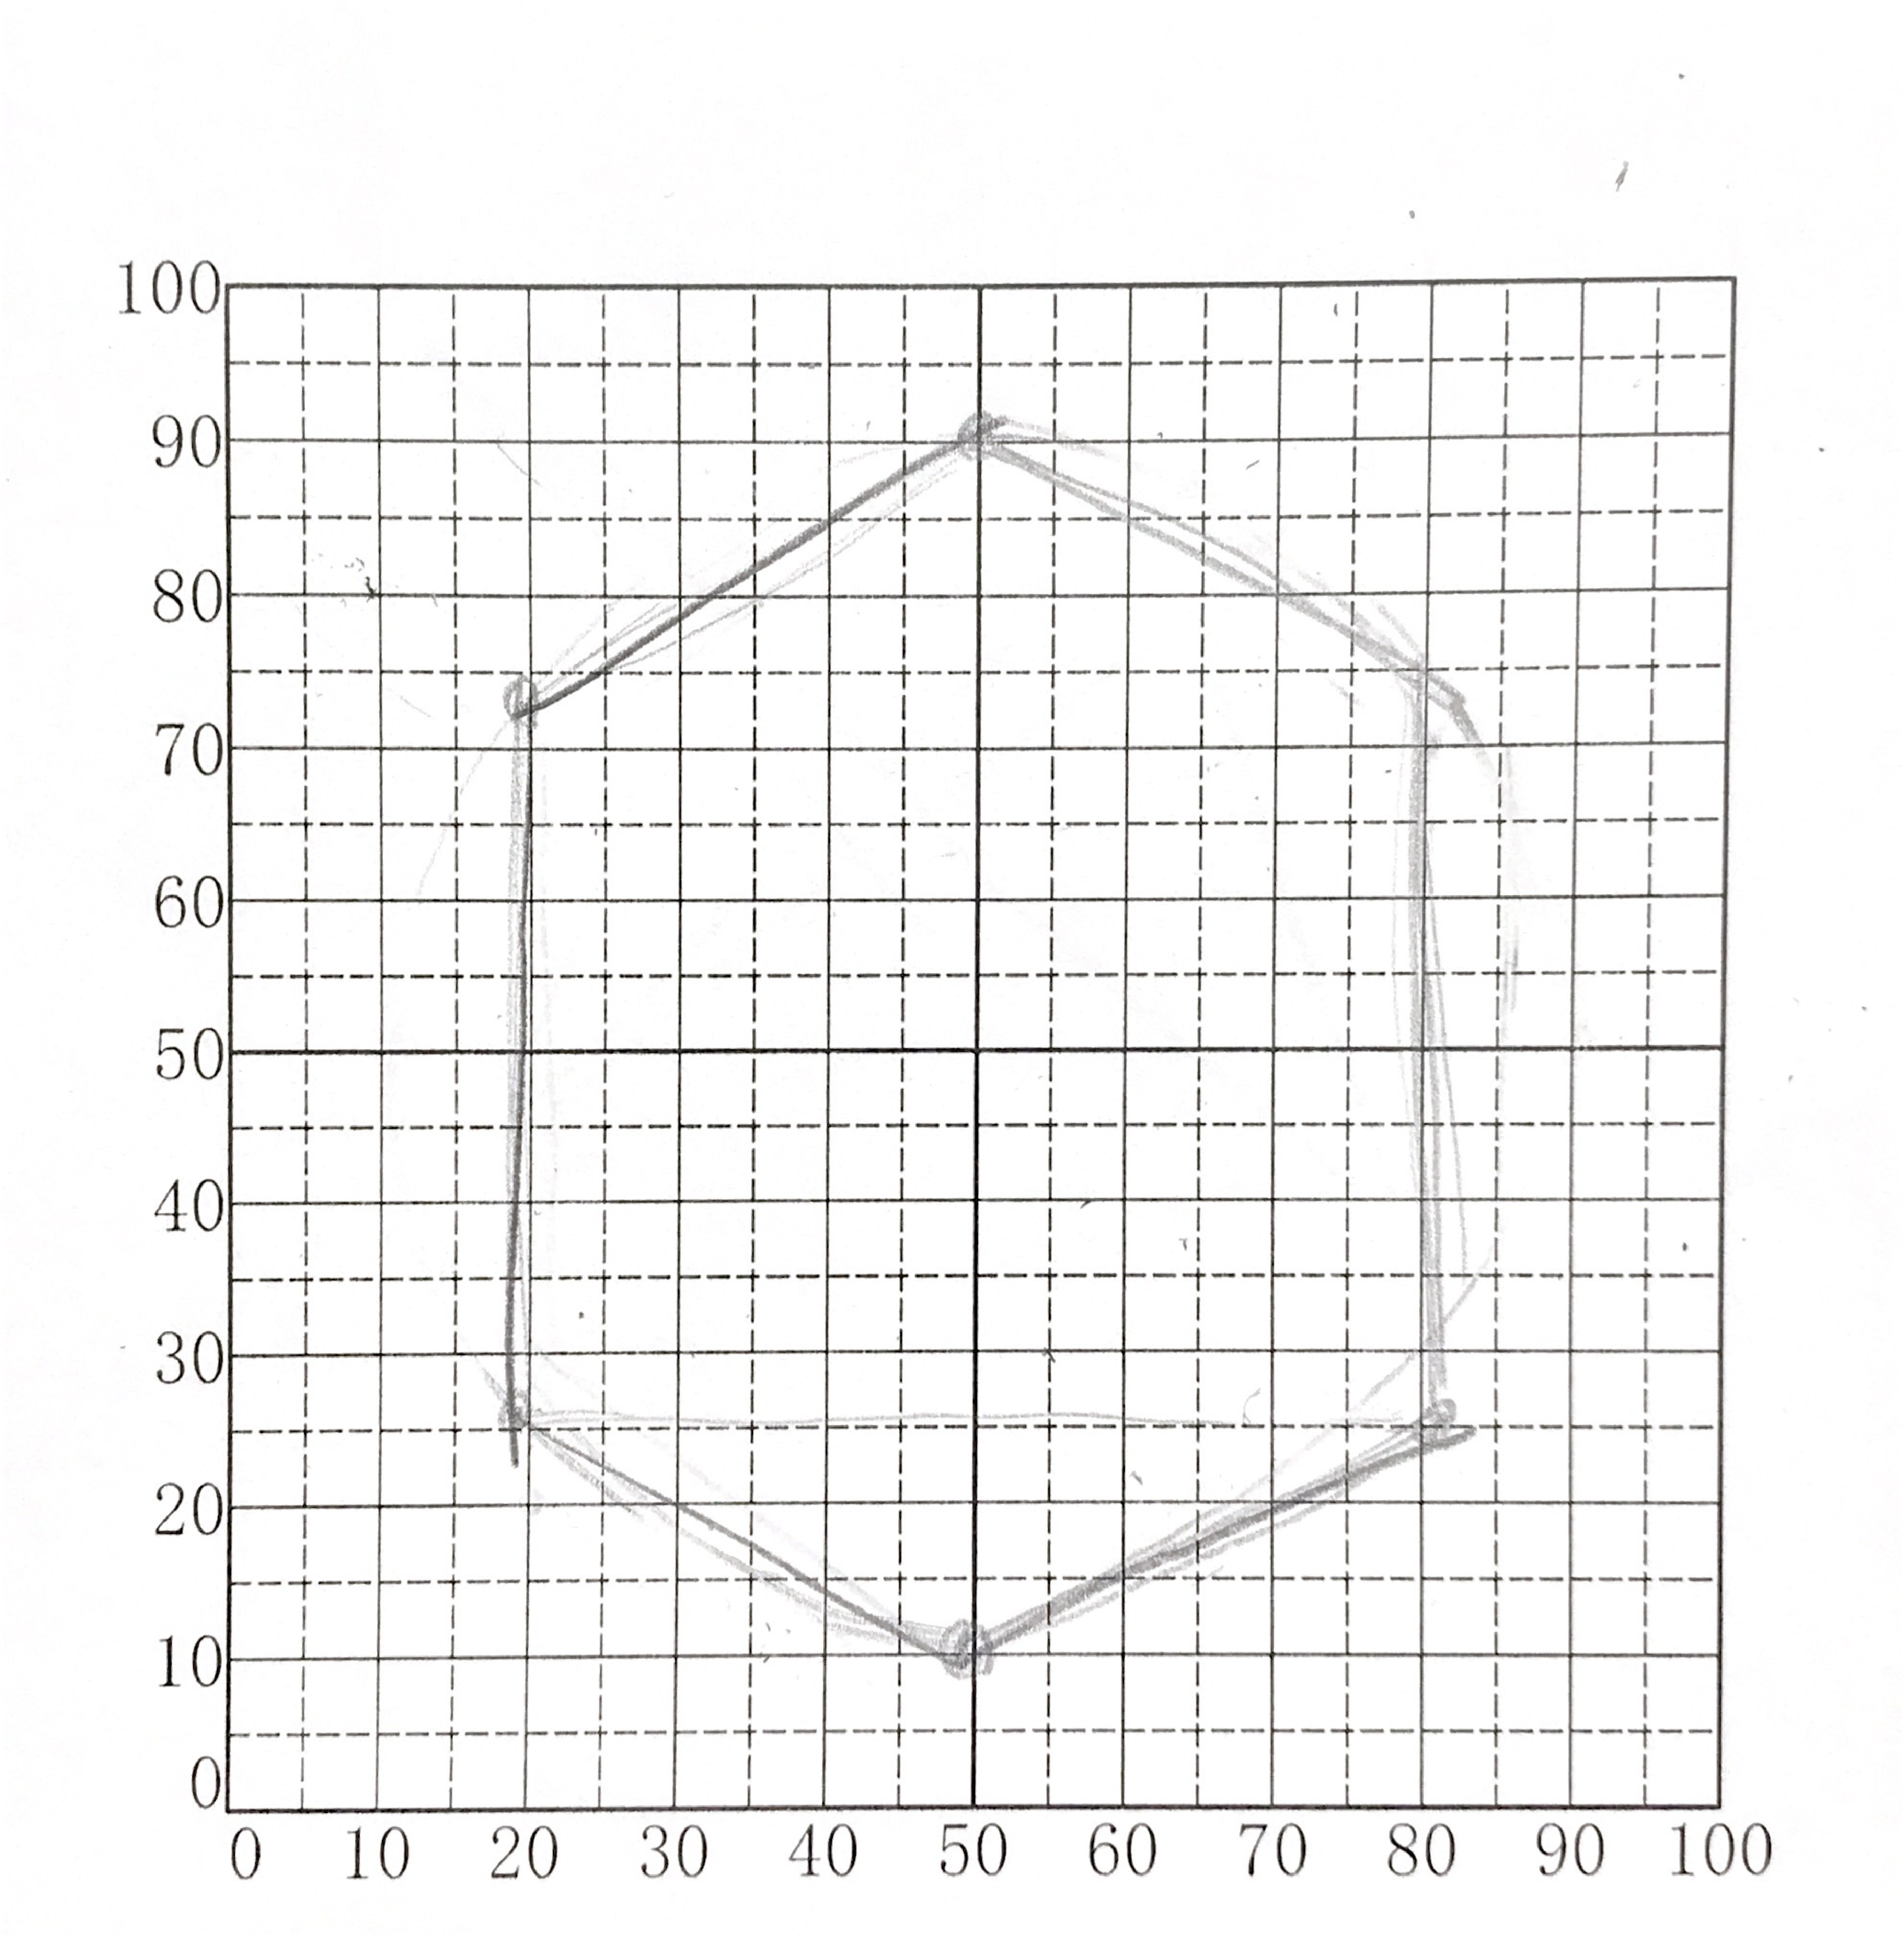
\includegraphics[width=5cm]{8_6.pdf}
    \caption{六角形}
    \label{fig:my_label}
\end{figure}
得られたデータは表13である。

\begin{table}[H]
    \centering
    \caption{六角形}
    \begin{tabular}{c|c}
       X座標&Y座標 \\
    \hline\hline
    22 &16 \\
     22&81\\
    54&92\\
   88 &65\\
    77&15\\
    44&7\\
    \end{tabular}
    
    \label{tab:my_label}
\end{table}

描画した結果は図22である。

\begin{figure}[H]
    \centering
    
    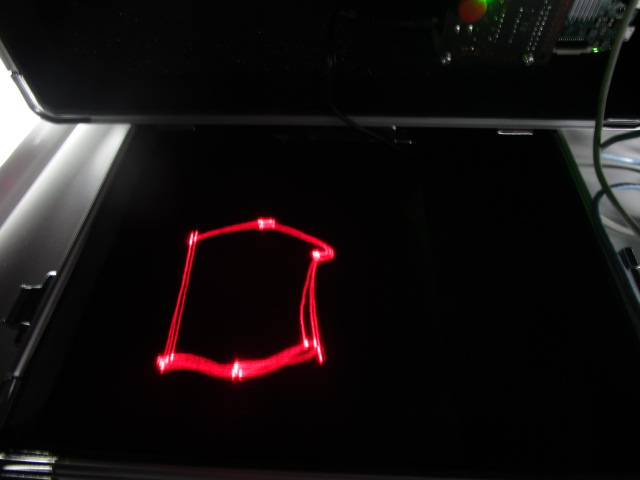
\includegraphics[width=5cm]{IMG_1756.JPG}
    \caption{六角形の描画}
    \label{fig:my_label}
\end{figure}

\subsection{結果(八角形)}

描画させる図形の方眼紙の図は図23である。
\begin{figure}[H]
    \centering
    
    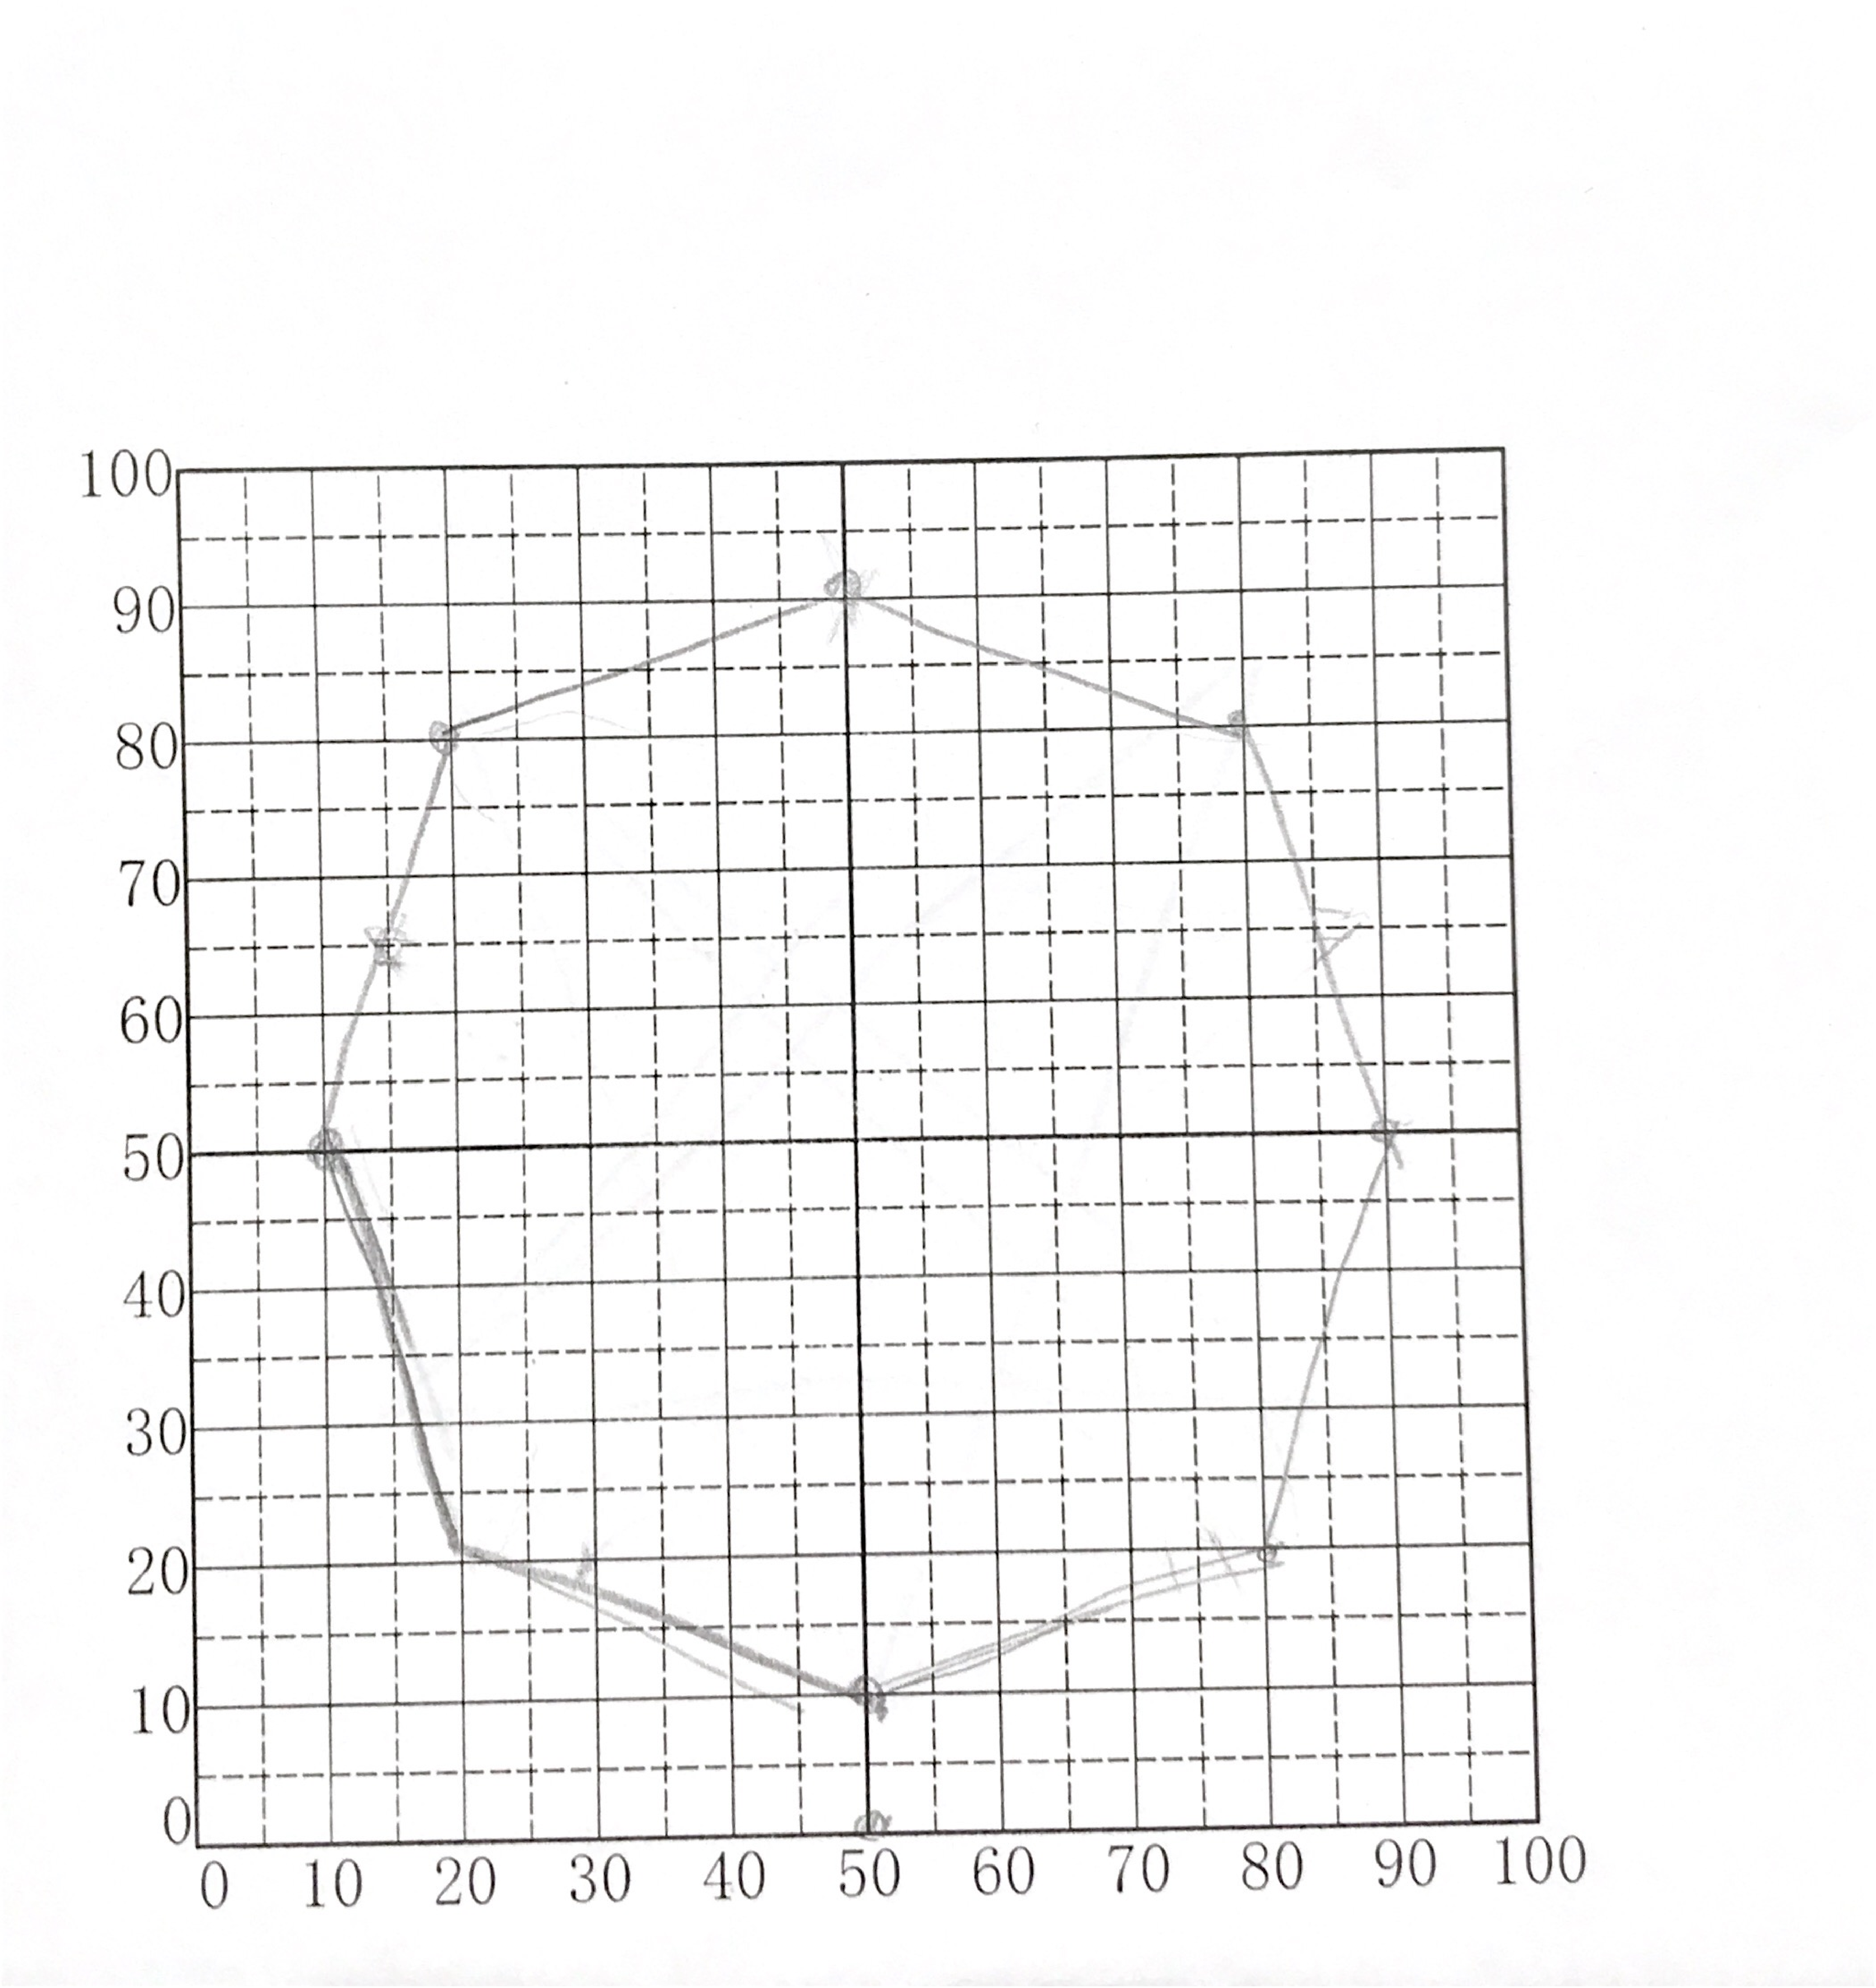
\includegraphics[width=5cm]{8_8.pdf}
    \caption{八角形}
    \label{fig:my_label}
\end{figure}


得られたデータは表14である。
\begin{table}[H]
    \centering
    \caption{八角形}
    \begin{tabular}{c|c}
       X座標&Y座標 \\
    \hline\hline
    50 &0 \\
    17 &11\\
    8&43\\
    22&83\\
    52&88\\
    93&68\\
    100&29\\
    78&10\\
    \end{tabular}
    
    \label{tab:my_label}
\end{table}
描画した結果は図24である。
\begin{figure}[H]
    \centering
    
    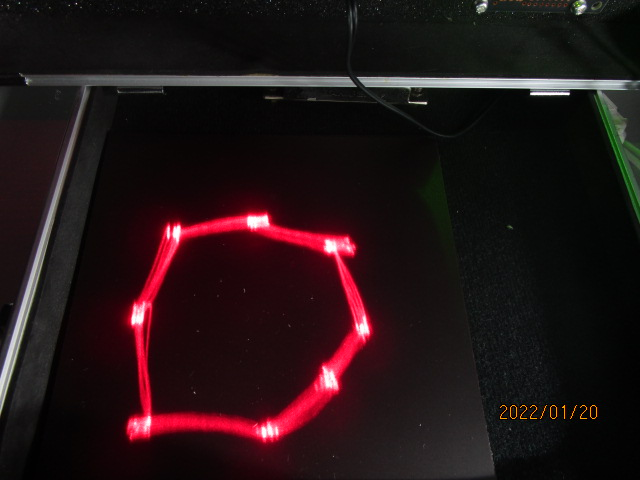
\includegraphics[width=5cm]{IMG_2194.JPG}
    \caption{八角形の描画}
    \label{fig:my_label}
\end{figure}\\
\subsection{結果(五芒星)}

描画させる図形の方眼紙の図は図25である。
\begin{figure}[H]
    \centering
    
    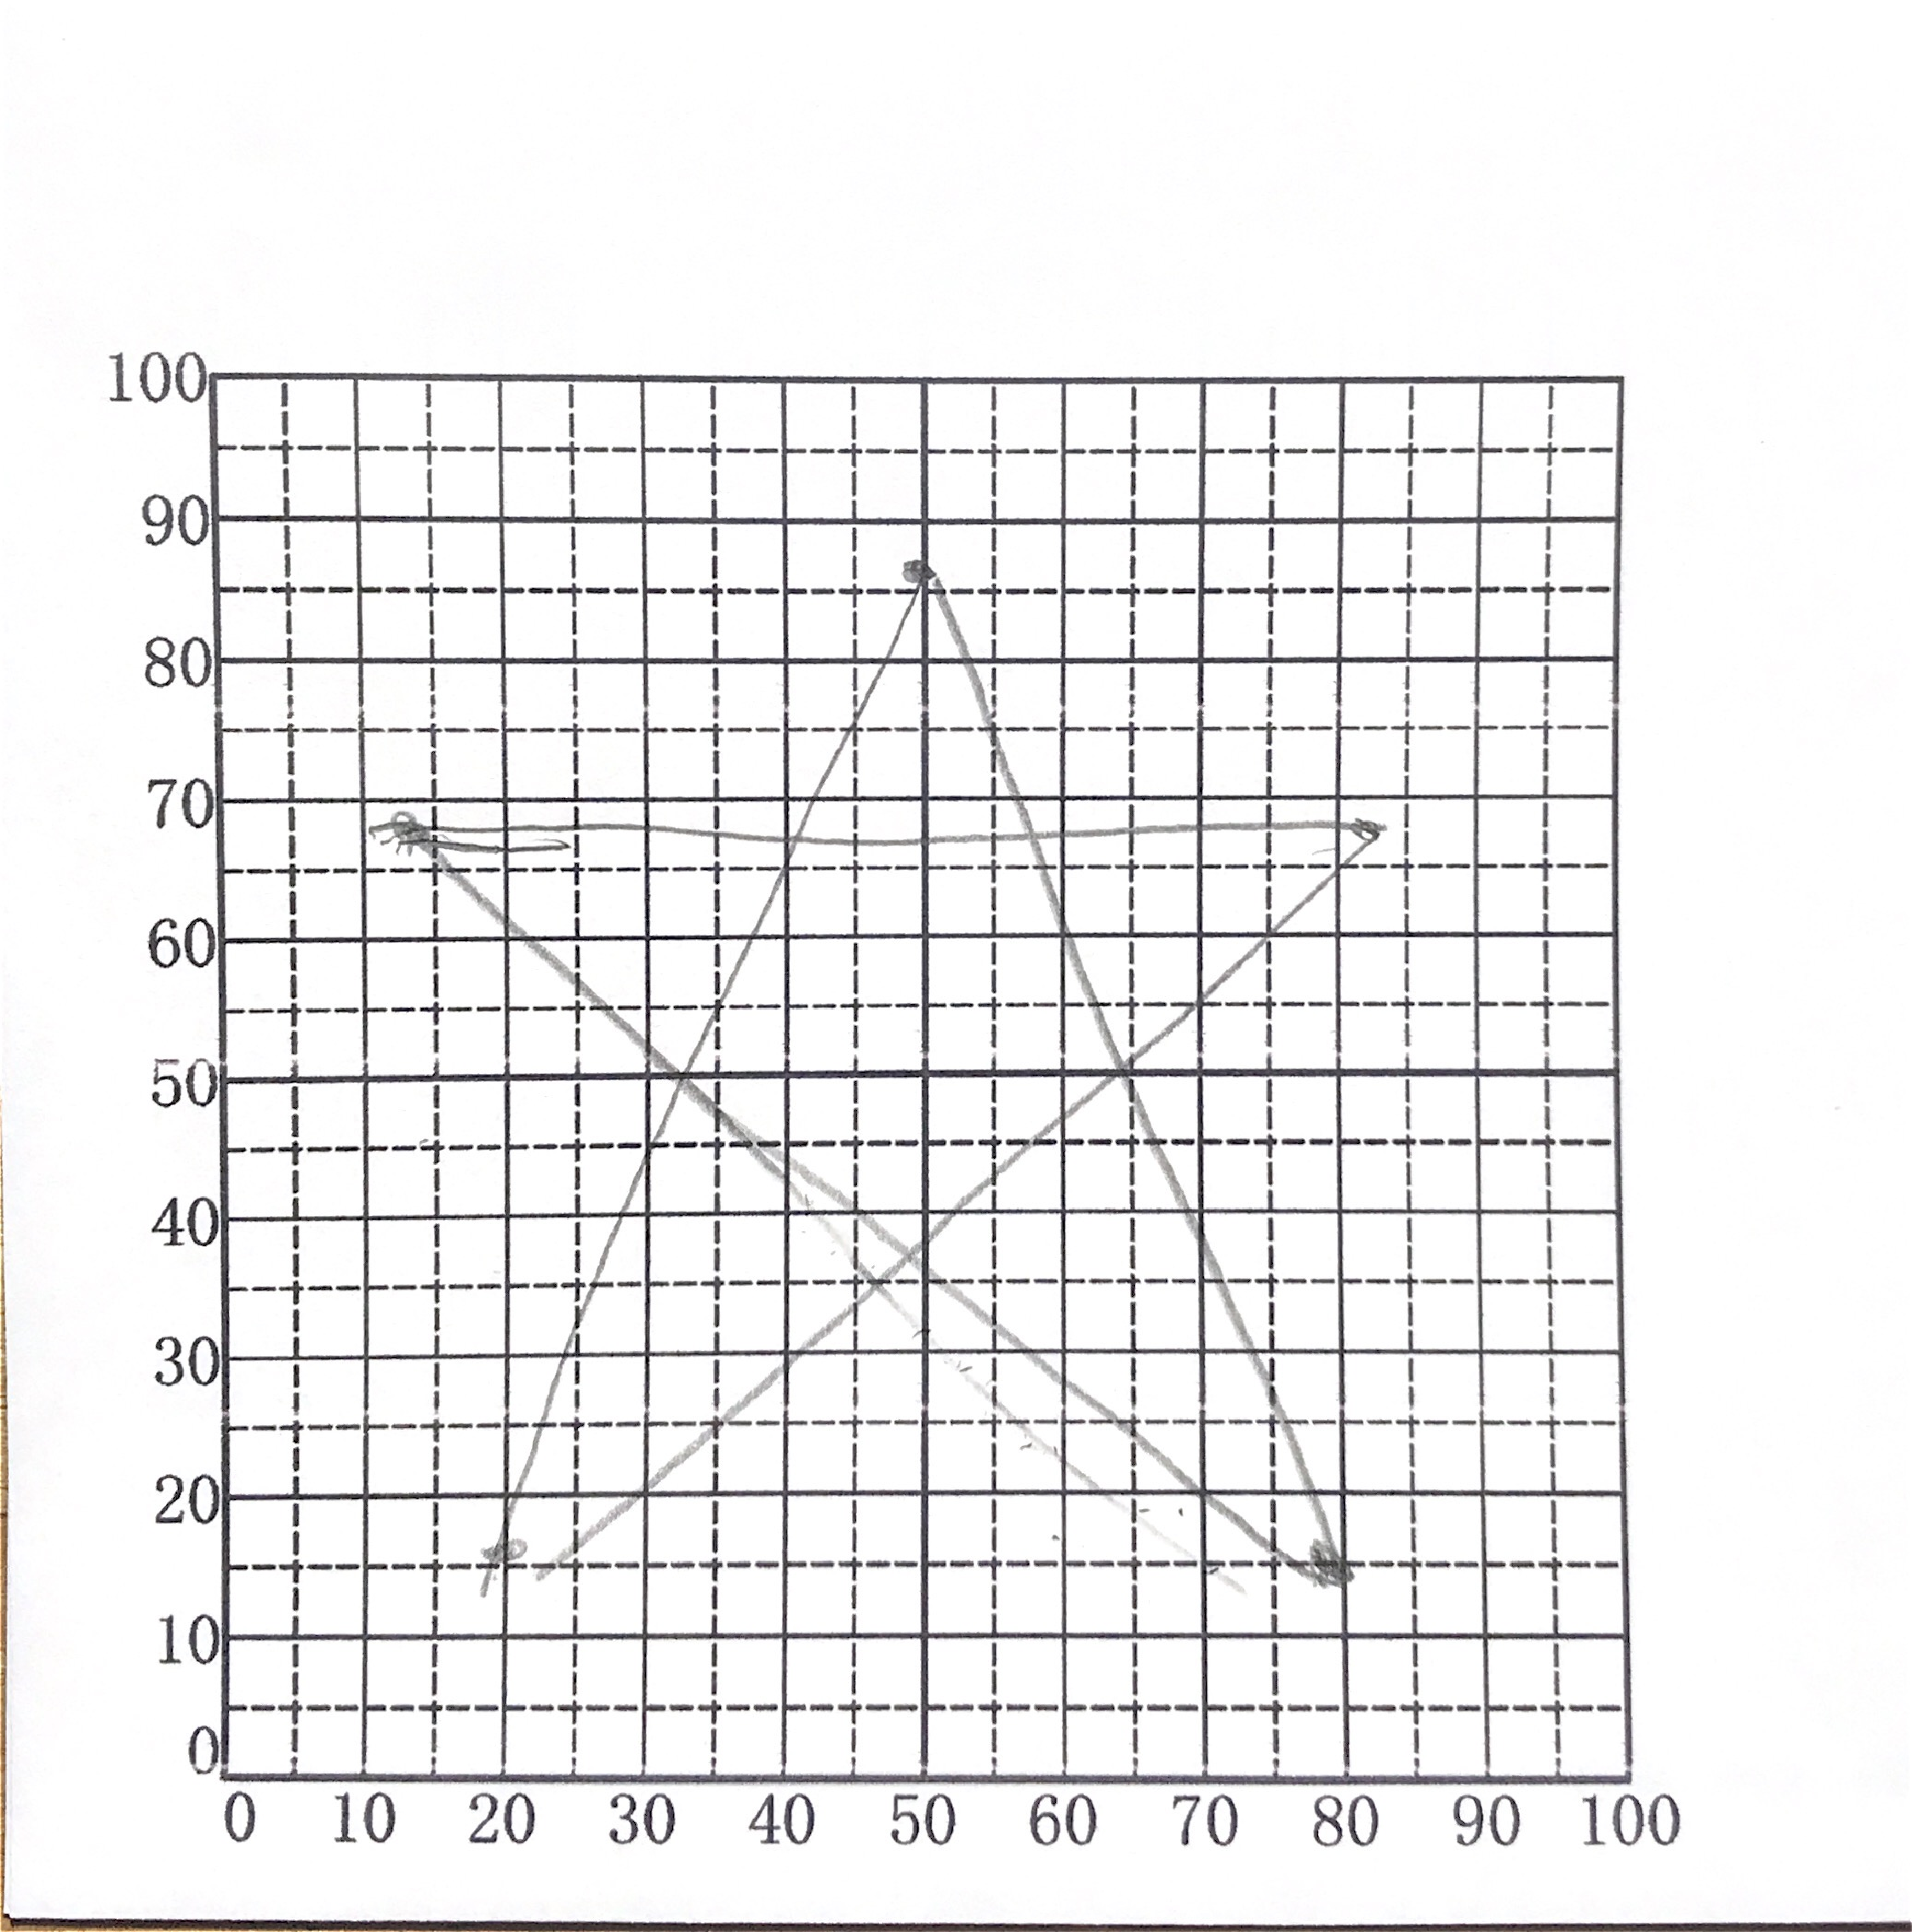
\includegraphics[width=5cm]{8_star.pdf}
    \caption{五芒星}
    \label{fig:my_label}
\end{figure}

得られたデータは表25である。
\begin{table}[H]
    \centering
    \caption{五芒星}
    \begin{tabular}{c|c}
       X座標&Y座標 \\
    \hline\hline
    48 &82 \\
    27 &10\\
    95&45\\
    11&56\\
    74&12\\
    
    \end{tabular}
    
    \label{tab:my_label}
\end{table}
描画したデータは図26である。
\begin{figure}[H]
    \centering
    
    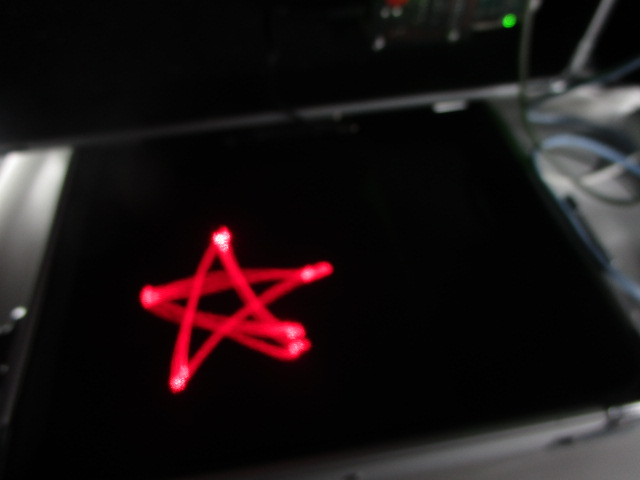
\includegraphics[width=5cm]{IMG_1758.JPG}
    \caption{五芒星の描画}
    \label{fig:my_label}
\end{figure}

\\
\subsection{考察}

八角形の描画を見ると、頂点近くでレーザ光が鋭角に動いたような跡がある。
このことから、レーザ光は斜めに動くため
、指定された頂点になるよう修正され指定された頂点になると考えられる。


\section{課題9}
\subsection{目的}
描画領域に円を書く。

\subsection{フロウチャート}

\begin{figure}[H]
    \centering
    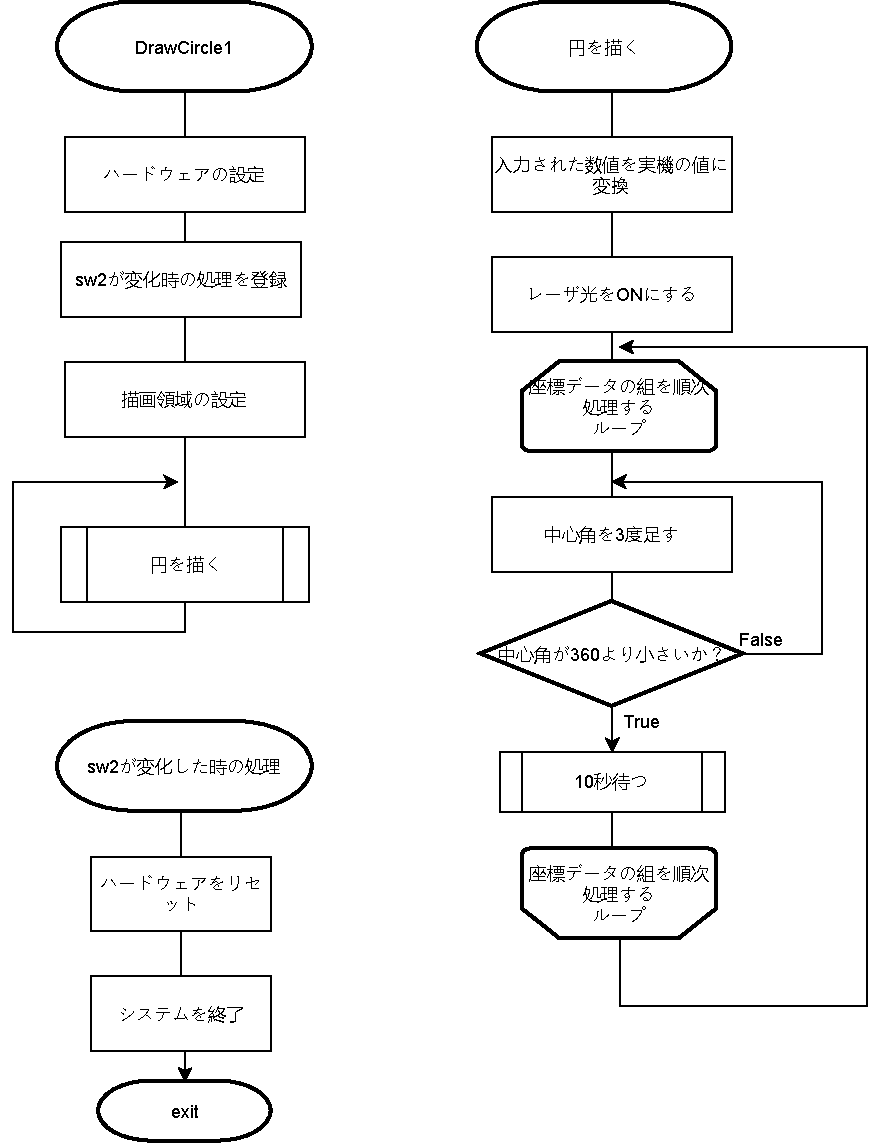
\includegraphics[scale=0.6]{kumikomiKadai9.pdf}
    \caption{課題9のフロウチャート}
    \label{fig:my_label}
\end{figure}

\subsection{実験方法}
\begin{lstlisting}[caption=DrawCircle1]
  import hardware.*;  //実験で実機を使用する場合にはコメントを外してこれを使用する
//import stub.*;  //予習などで実機を使用せずに動作を確認する場合には、これを使用する

public class Kadai9_DrawCircle1
{
    private Hardware hardware = Hardware.getInstance(); //ハードウェアのインスタンスを取得する

    public void drawFigure() {
        System.out.println( "Start!" );
        hardware.manipulator.sw2.addListener( () -> systemExit() );

        hardware.drawUnit.servoX.setMinMax(    119,213    ); //X座標の最小値と最大値を入れる
        hardware.drawUnit.servoY.setMinMax(  29  ,  140  ); //Y座標の最小値と最大値を入れる

        double r = 40 ;     // 半径 r
        double x0 = 50  ;    // 中心座標 x0
        double y0 =  50 ;    // 中心座標 y0
        hardware.drawUnit.laser.on();

        while ( true ) {
            for ( int th=0 ; th<360 ; th += 3 ) { //中心角を3°間隔で360°回す
                double radian = Math.toRadians( th );
                double x = x0 + r * Math.cos( radian );
                double y = y0 + r * Math.sin( radian );
                hardware.drawUnit.servoX.setValue( convertX( (int)x ) );
                hardware.drawUnit.servoY.setValue( convertY( (int)y ) );
                UtilityTools.wait_ms( 10 );
            }
        }
    }

    private int convertX( int x ) {
        int xMin = hardware.drawUnit.servoX.getMin();
        int xMax = hardware.drawUnit.servoX.getMax();
        double X=x*(xMax-xMin)/100+xMin;
        return (  (int)X  );  //この部分に変換式を記述する
    }

    private int convertY( int y ) {
        int yMin = hardware.drawUnit.servoY.getMin();
        int yMax = hardware.drawUnit.servoY.getMax();
        double Y=y*(yMax-yMin)/100+yMin;
        return ( (int)Y  );  //この部分に変換式を記述する
    }

    private void systemExit() {
        hardware.reset();
        System.out.println( "End!." );
        System.exit( 0 );
    }
}

\end{lstlisting}

\newpage
\subsection{結果}



\begin{figure}[h]
    \centering
    
    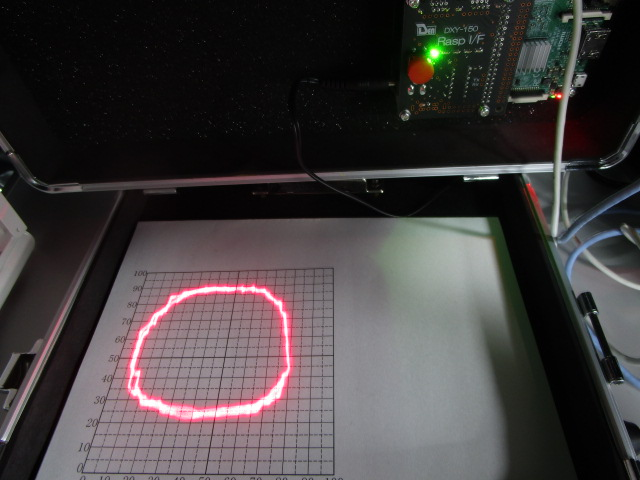
\includegraphics[width=5cm]{IMG_1740.JPG}
    \caption{課題9結果}
    \label{fig:my_label}
\end{figure}

\subsection{考察}

課題9の時と同様に斜めに動いたのちに指定された値に修正しているため、ギザギザしたと考えられる。

\section{課題10}


\subsection{目的}
描画領域に同心円を描く。

\subsection{フロウチャート}

\begin{figure}[H]
    \centering
    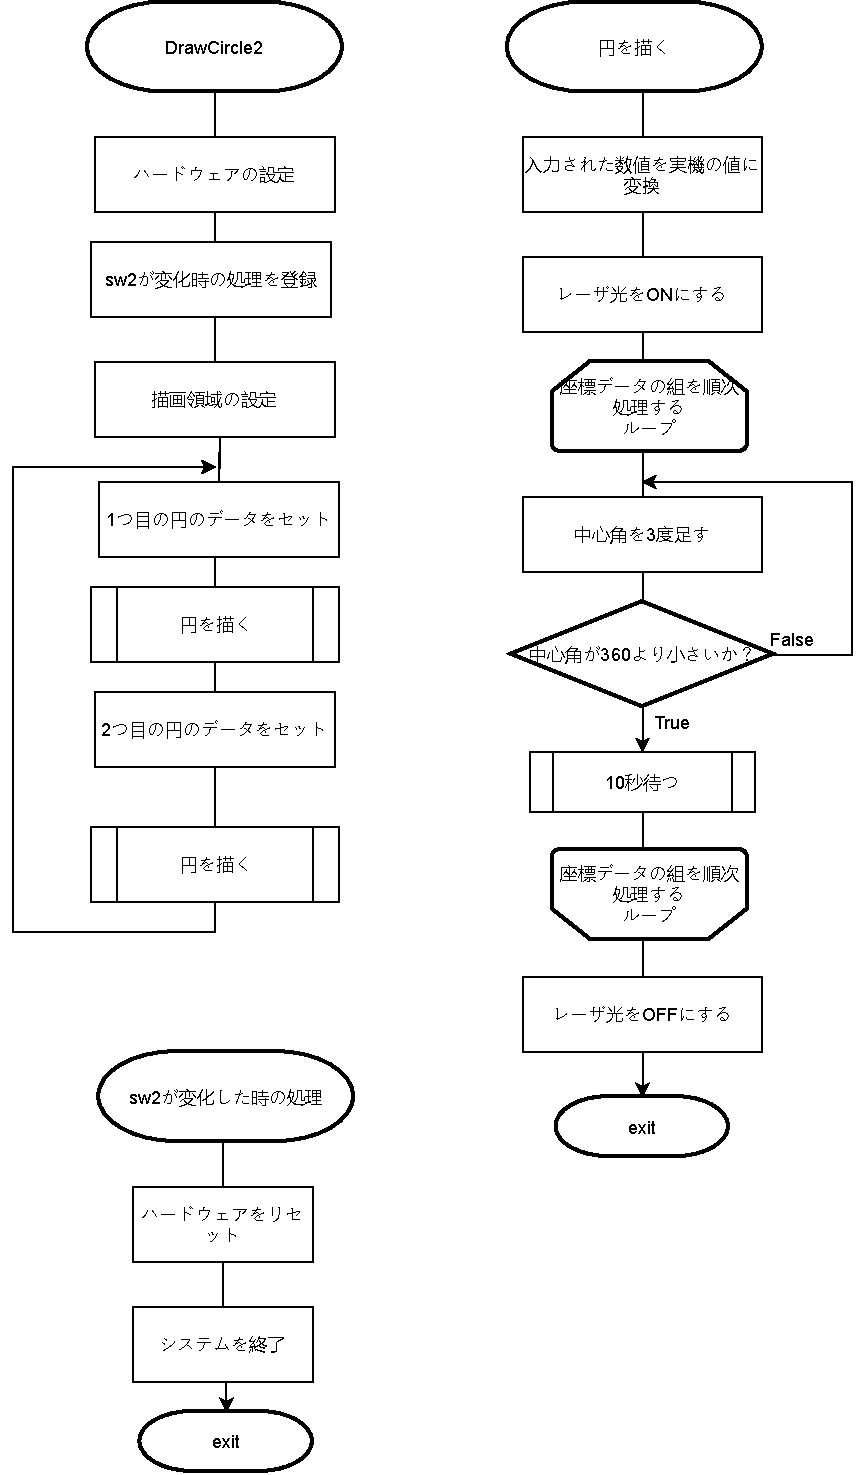
\includegraphics{kumikomiKadai10.pdf}
    \caption{課題10のフロウチャート}
    \label{fig:my_label}
\end{figure}

\subsection{実験方法}
\begin{lstlisting}[caption=DrawCircle]

//import hardware.*;  //実験で実機を使用する場合にはコメントを外してこれを使用する
import stub.*;  //予習などで実機を使用せずに動作を確認する場合には、これを使用する

public class Kadai10_DrawCircle2
{
    private Hardware hardware = Hardware.getInstance(); //ハードウェアのインスタンスを取得する

    public void drawFigure() {
        System.out.println( "Start!" );
        hardware.manipulator.sw2.addListener( () -> systemExit() );

        hardware.drawUnit.servoX.setMinMax( 0,100 ); //X座標の最小値と最大値を入れる
        hardware.drawUnit.servoY.setMinMax( 0 ,100 ); //Y座標の最小値と最大値を入れる

        double r = 20  ;     // 半径 r1

        double x0 = 50  ;    // 中心座標 x0
        double y0 =  50 ;    // 中心座標 y0
        
        hardware.drawUnit.laser.on();
        for ( int th=0 ; th<360 ; th += 3 ) { //中心角を3°間隔で360°回す
            double radian = Math.toRadians( th );
            double x = x0 + r * Math.cos( radian );
            double y = y0 + r * Math.sin( radian );
            hardware.drawUnit.servoX.setValue( convertX( (int)x ) );
            hardware.drawUnit.servoY.setValue( convertY( (int)y ) );
            UtilityTools.wait_ms( 10 );
        }
        hardware.drawUnit.laser.off();
        UtilityTools.wait_ms( 10 );
        double r2 = 40  ;     //半径r2
        hardware.drawUnit.laser.on();
        for ( int th=0 ; th<360 ; th += 3 ) { //中心角を3°間隔で360°回す
            double radian = Math.toRadians( th );
            double x = x0 + r2 * Math.cos( radian );
            double y = y0 + r2 * Math.sin( radian );
            hardware.drawUnit.servoX.setValue( convertX( (int)x ) );
            hardware.drawUnit.servoY.setValue( convertY( (int)y ) );
            UtilityTools.wait_ms( 10 );
        }
        hardware.drawUnit.laser.off();
    }
    private int convertX( int x ) {
        int xMin = hardware.drawUnit.servoX.getMin();
        int xMax = hardware.drawUnit.servoX.getMax();
        double X=x*(xMax-xMin)/100+xMin;
        return (  (int)X  );  
    }

    private int convertY( int y ) {
        int yMin = hardware.drawUnit.servoY.getMin();
        int yMax = hardware.drawUnit.servoY.getMax();
        double Y=y*(yMax-yMin)/100+yMin;
        return ( (int)Y  );  
    }

    private void systemExit() {
        hardware.reset();
        System.out.println( "End!." );
        System.exit( 0 );
    }

}

\end{lstlisting}

\subsection{結果}

\begin{figure}[H]
    \centering
    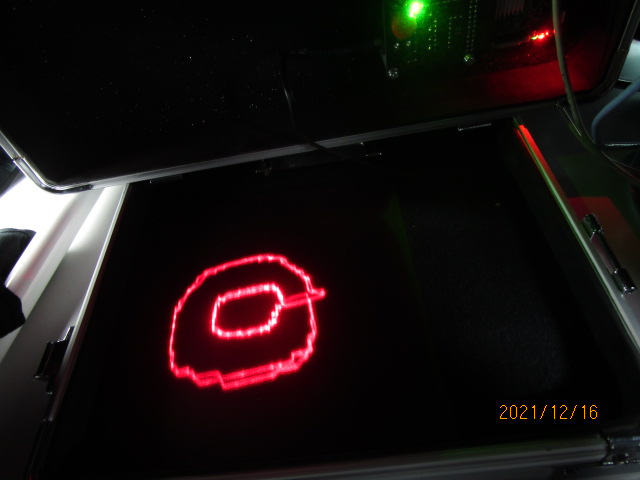
\includegraphics[width=5cm]{IMG_2154.JPG}
    \caption{同心円の描画}
    \label{fig:my_label}
\end{figure}

円と円の間を移動する際にレーザ光がOFFにならずに失敗してしまった。


\subsubsection{考察}

コードではレーザ光をOFFにしたのち次の円にいき、レーザ光をふたたびONにしているが、実際にはレーザ光をOFFにする動きが行われなかったと考えられる。
whileでループさせている部分に現在は単に

\section{課題11}

\subsection{目的}

\subsection{フロウチャート}

\subsection{実験方法}

\subsection{結果}




\section{課題12}

\subsection{目的}

\subsection{フロウチャート}

\subsection{実験方法}

\subsection{結果}



\section{課題13}


\subsection{目的}

\subsection{フロウチャート}

\subsection{実験方法}

\subsection{結果}


\section{まとめ}

\end{document}
